\documentclass[12pt]{article}
\usepackage{blindtext}
\usepackage{geometry}
\geometry{
	a4paper,
	left=40mm,
	right=15mm,
	top=30mm,
	bottom=35mm,
 }
\usepackage{setspace}
% Seznam balíků
\usepackage{comment}
\usepackage{lmodern}
\usepackage{cmap}
\usepackage[czech]{babel}
\usepackage[T1]{fontenc}
\usepackage[utf8]{inputenc}
\usepackage{graphicx}
\usepackage{epstopdf}
\usepackage{makeidx}
\usepackage{listings}
\usepackage[export]{adjustbox}
\usepackage[font=scriptsize,labelfont=bf]{caption}
\usepackage{booktabs}
\usepackage{subcaption}
\usepackage{array}
\usepackage{multirow}
\usepackage{enumitem}
\usepackage{tocbibind}
\usepackage{courier}
\usepackage{pdfpages}
\usepackage{float}
\usepackage{hyperref}
\hypersetup{
	colorlinks,
	citecolor=black,
	filecolor=black,
	linkcolor=black,
	urlcolor=black
}
\usepackage{times}
\graphicspath{{./images/}}

% Začátek dokumentu
\begin{document}
	% Titulní stránka
	\begin{titlepage}
		\centering
		\fontfamily{lmss}\selectfont
		\begin{tabular}{m{0.2\linewidth}m{0.8\linewidth}}
			
\includegraphics[width=\linewidth]{SPSE_logo}
			&\centering
			\textbf{Vyšší odborná škola}\par
			\textbf{a Střední průmyslová škola elektrotechnická}\par
			\textbf{Plzeň, Koterovská 85}
		\end{tabular}
		\centering
		\vfill
		{\Huge\sc\textsf{\textbf{Ročníková práce}}\par}
		\raggedright
		\vspace{4cm}
		{\Large Téma: \textbf{Programovatelné auto}\par}
		\vfill
		
		% Spodní část titulní stránky
		\textbf{\begin{tabular}{ll}
			Autor práce:		&	Jan Ocelík \\
			Obor studia:		&	78-42-M/01 Technické lyceum \\
			Třída:				&	3. L \\
			Předmět:			&	Kybernetika \\
			Zadávající učitel:	&	Jiří Švihla \\
			Dne:				&	28. 4. 2023 \\
								&	\\
			Hodnocení:			&	\\
		\end{tabular}}
	\end{titlepage}

	% Zadání
	\thispagestyle{empty}
	\includepdfset{offset=15mm 0mm,noautoscale,pages={-},pagecommand={}}
	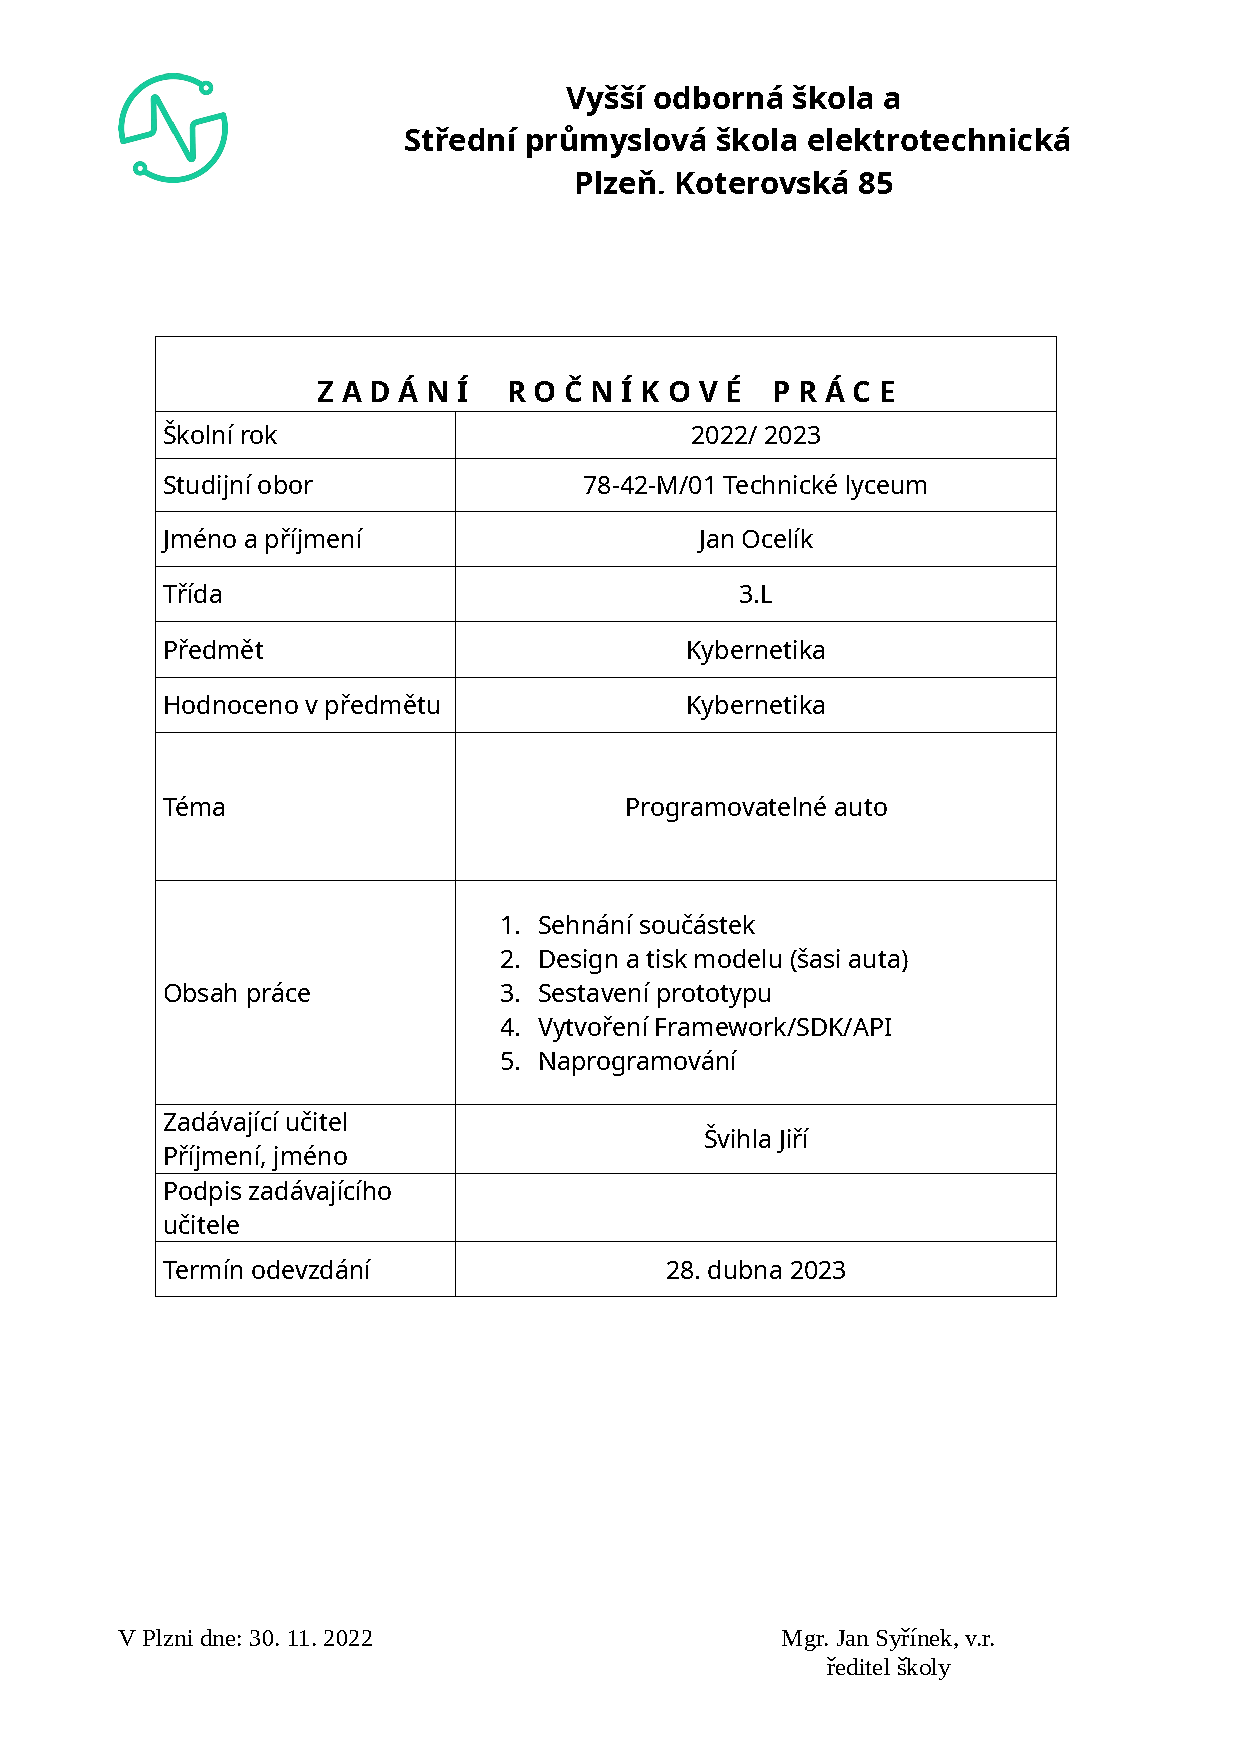
\includepdf[pages=1]{Zadani_RP_TL_22_23.pdf}
	
	\begin{spacing}{1.5}
	
	% Anotace
	\newpage
	\thispagestyle{empty}
	\section*{Anotace}
	\addcontentsline{toc}{section}{Anotace}
	\paragraph{} Cílem této ročníkové práce je za pomoci opensource programů navrhnout a z opensource komponent poskládat robotické autíčko pro začátečníky i pokročilé s možností jednoduchého sestavení. Dalším úkolem je vyvinout firmware a API pro jednoduché skriptové programovaní i komplexnější programování s využitím obrazového vstupu. Dalším úkolem je připravit ukázkové příklady kódu k předvedení jednotlivých funkcí robota. Posledním úkolem je zpříjemnit práci s robotem, zhodnotit přínosy a možnosti využití projektu ve vzdělávání a vypracovat potřebnou dokumentaci.
	\vfill
	\paragraph{} „Prohlašuji, že jsem tuto práci vypracoval samostatně a použil literárních pramenů a informací, které cituji a uvádím v seznamu použité literatury a zdrojů informací.“
	\paragraph{} „Souhlasím s využitím mé práce učiteli VOŠ a SPŠE Plzeň k výuce.“
	\paragraph{} \hfill Plzni dne: .................... Podpis: ....................
	
	% Poděkování
	\newpage
	\thispagestyle{empty}
	\section*{Poděkování}
	\addcontentsline{toc}{section}{Poděkování}
	\paragraph{} Tímto bych chtěl poděkovat vedoucímu práce Jiřímu Švihlovi za pomoc s výběrem komponent a obsahem dokumentace a rodině a přátelům za psychickou podporu. Také děkuji všem dohromady za to, že mě k tomu včas dokopali.
	
	% Obsah
	\newpage
	\tableofcontents
	
	% Úvod
	\newpage
	\section{Úvod}
	\paragraph{} V dnešní době se stále více hovoří o automatizaci a digitalizaci a tyto trendy mají velký vliv na společnost. Robotika a autonomní systémy jsou jednou z klíčových oblastí, které se rozvíjejí v rámci těchto trendů a mají potenciál změnit mnoho aspektů našeho života.
	\paragraph{} Vzdělávání a výuka v této oblasti se také stávají stále důležitějšími, protože mnoho pracovních pozic, které budou v budoucnosti vyžadovat znalosti robotiky a programování, ještě neexistuje. Výuka v této oblasti tak může být klíčová pro přípravu studentů na pracovní trh budoucnosti.
	\paragraph{} Proto jsem se rozhodl věnovat svou ročníkovou práci právě problematice robotiky a vytvořit autonomní auto, které bude sloužit jako výuková pomůcka. Můj záměr je ukázat, jak moderní technologie mohou být využity k tomu, aby byli studenti lépe připraveni na budoucí výzvy v oblasti robotiky a informatiky.
	\paragraph{} Při tvorbě prototypu se budu snažit využít nejnovější poznatky v oblasti robotiky a programování, a to jak z teoretického hlediska, tak z praktického testování. Cílem bude vytvořit zařízení, které bude snadno ovladatelné a srozumitelné pro studenty různých věkových kategorií, a zároveň bude dostatečně funkční a výkonné pro splnění zadaných úkolů.
	\paragraph{} Věřím, že tato ročníková práce přispěje k popularizaci robotiky a podpoří zájem studentů o tuto oblast. Tím může mít pozitivní vliv na jejich budoucí kariéru a na rozvoj robotiky v České republice.
	
	% Cíle a požadavky
	\newpage
	\subsection{Cíle a požadavky}
	
	\subsubsection{Komponenty (moduly)}
	\paragraph{} Hlavním cílem této ročníkové práce je návrh a výroba robota z běžně dostupných materiálů, v tomto případě ze snadno sehnatelných modulů.
	\paragraph{} Moduly by měly být zároveň opensource, aby si software pro ně mohl programovat každý, který se k robotovi dostane, nebo si ho sám vyrobí.
	\paragraph{} Důležitý je také výběr napájení, v případě robotického auta tedy baterie, tak, aby udrželo robota v provozu po přiměřeně dlouhou dobu a aby zároveň dokázalo vykrýt proudové špičky.
	
	\subsubsection{Šasi (tělo)}
	\paragraph{} Tělo robota by mělo být vyrobeno tak, aby bylo plně uzavíratelné, tedy bezpečné pro jakýkoli přenos i při nešetrném zacházení, ale aby se dal robot také provozovat s plně přístupnými veškerými propojkami a bylo tedy snadné ladit jeho hardware za provozu.
	
	\subsubsection{API}
	\paragraph{} Jedním z dalších požadavků je co nejvíce zpříjemnit uživateli práci s robotickým autem, tedy vytvořit nějaké API nebo knihovnu.
	\paragraph{} Nedílnou součástí je také dokumentace k danému API/knihovně a to proto, aby si i nově příchozí uživatel zvládl bez jakékoli pomoci robota pomocí daného API/knihovny naprogramovat.
	
	% Návrhový software
	\newpage
	\subsection{Návrhový software}
	
	\subsubsection{Onshape}
	\paragraph{} Onshape je online software pro návrh 3D součástí. V programu se vytváří takzvaný dokument, ve kterém se nadále dají zakládat \uv{studia}. Onshape nabízí mnoho zajímavých možností, běžného uživatele však zajímají tato tři hlavní studia - \textbf{Part Studio}, \textbf{Assembly} a \textbf{Drawing}.
	\subsubsection*{Part Studio}
	\paragraph{} Part Studio slouží, jak už název napovídá, k vytváření jednotlivých dílů. Díly se vytvářejí a upravují pomocí příkazů, jako například \textbf{Sketch} (sloužící k sestrojení 2D náčrtu), \textbf{Extrude} (\uv{vytáhnutí} náčrtu do třetího rozměru) nebo \textbf{Fillet} (zaoblení hran). Tyto příkazy lze vyvolat kliknutím na jejich ikonu v horní liště programu, přepsáním jejich názvu do \textbf{Search tools}, nebo, u některých více používaných, klávesovými zkratkami.
	
	\begin{figure}[H]
		\centering
		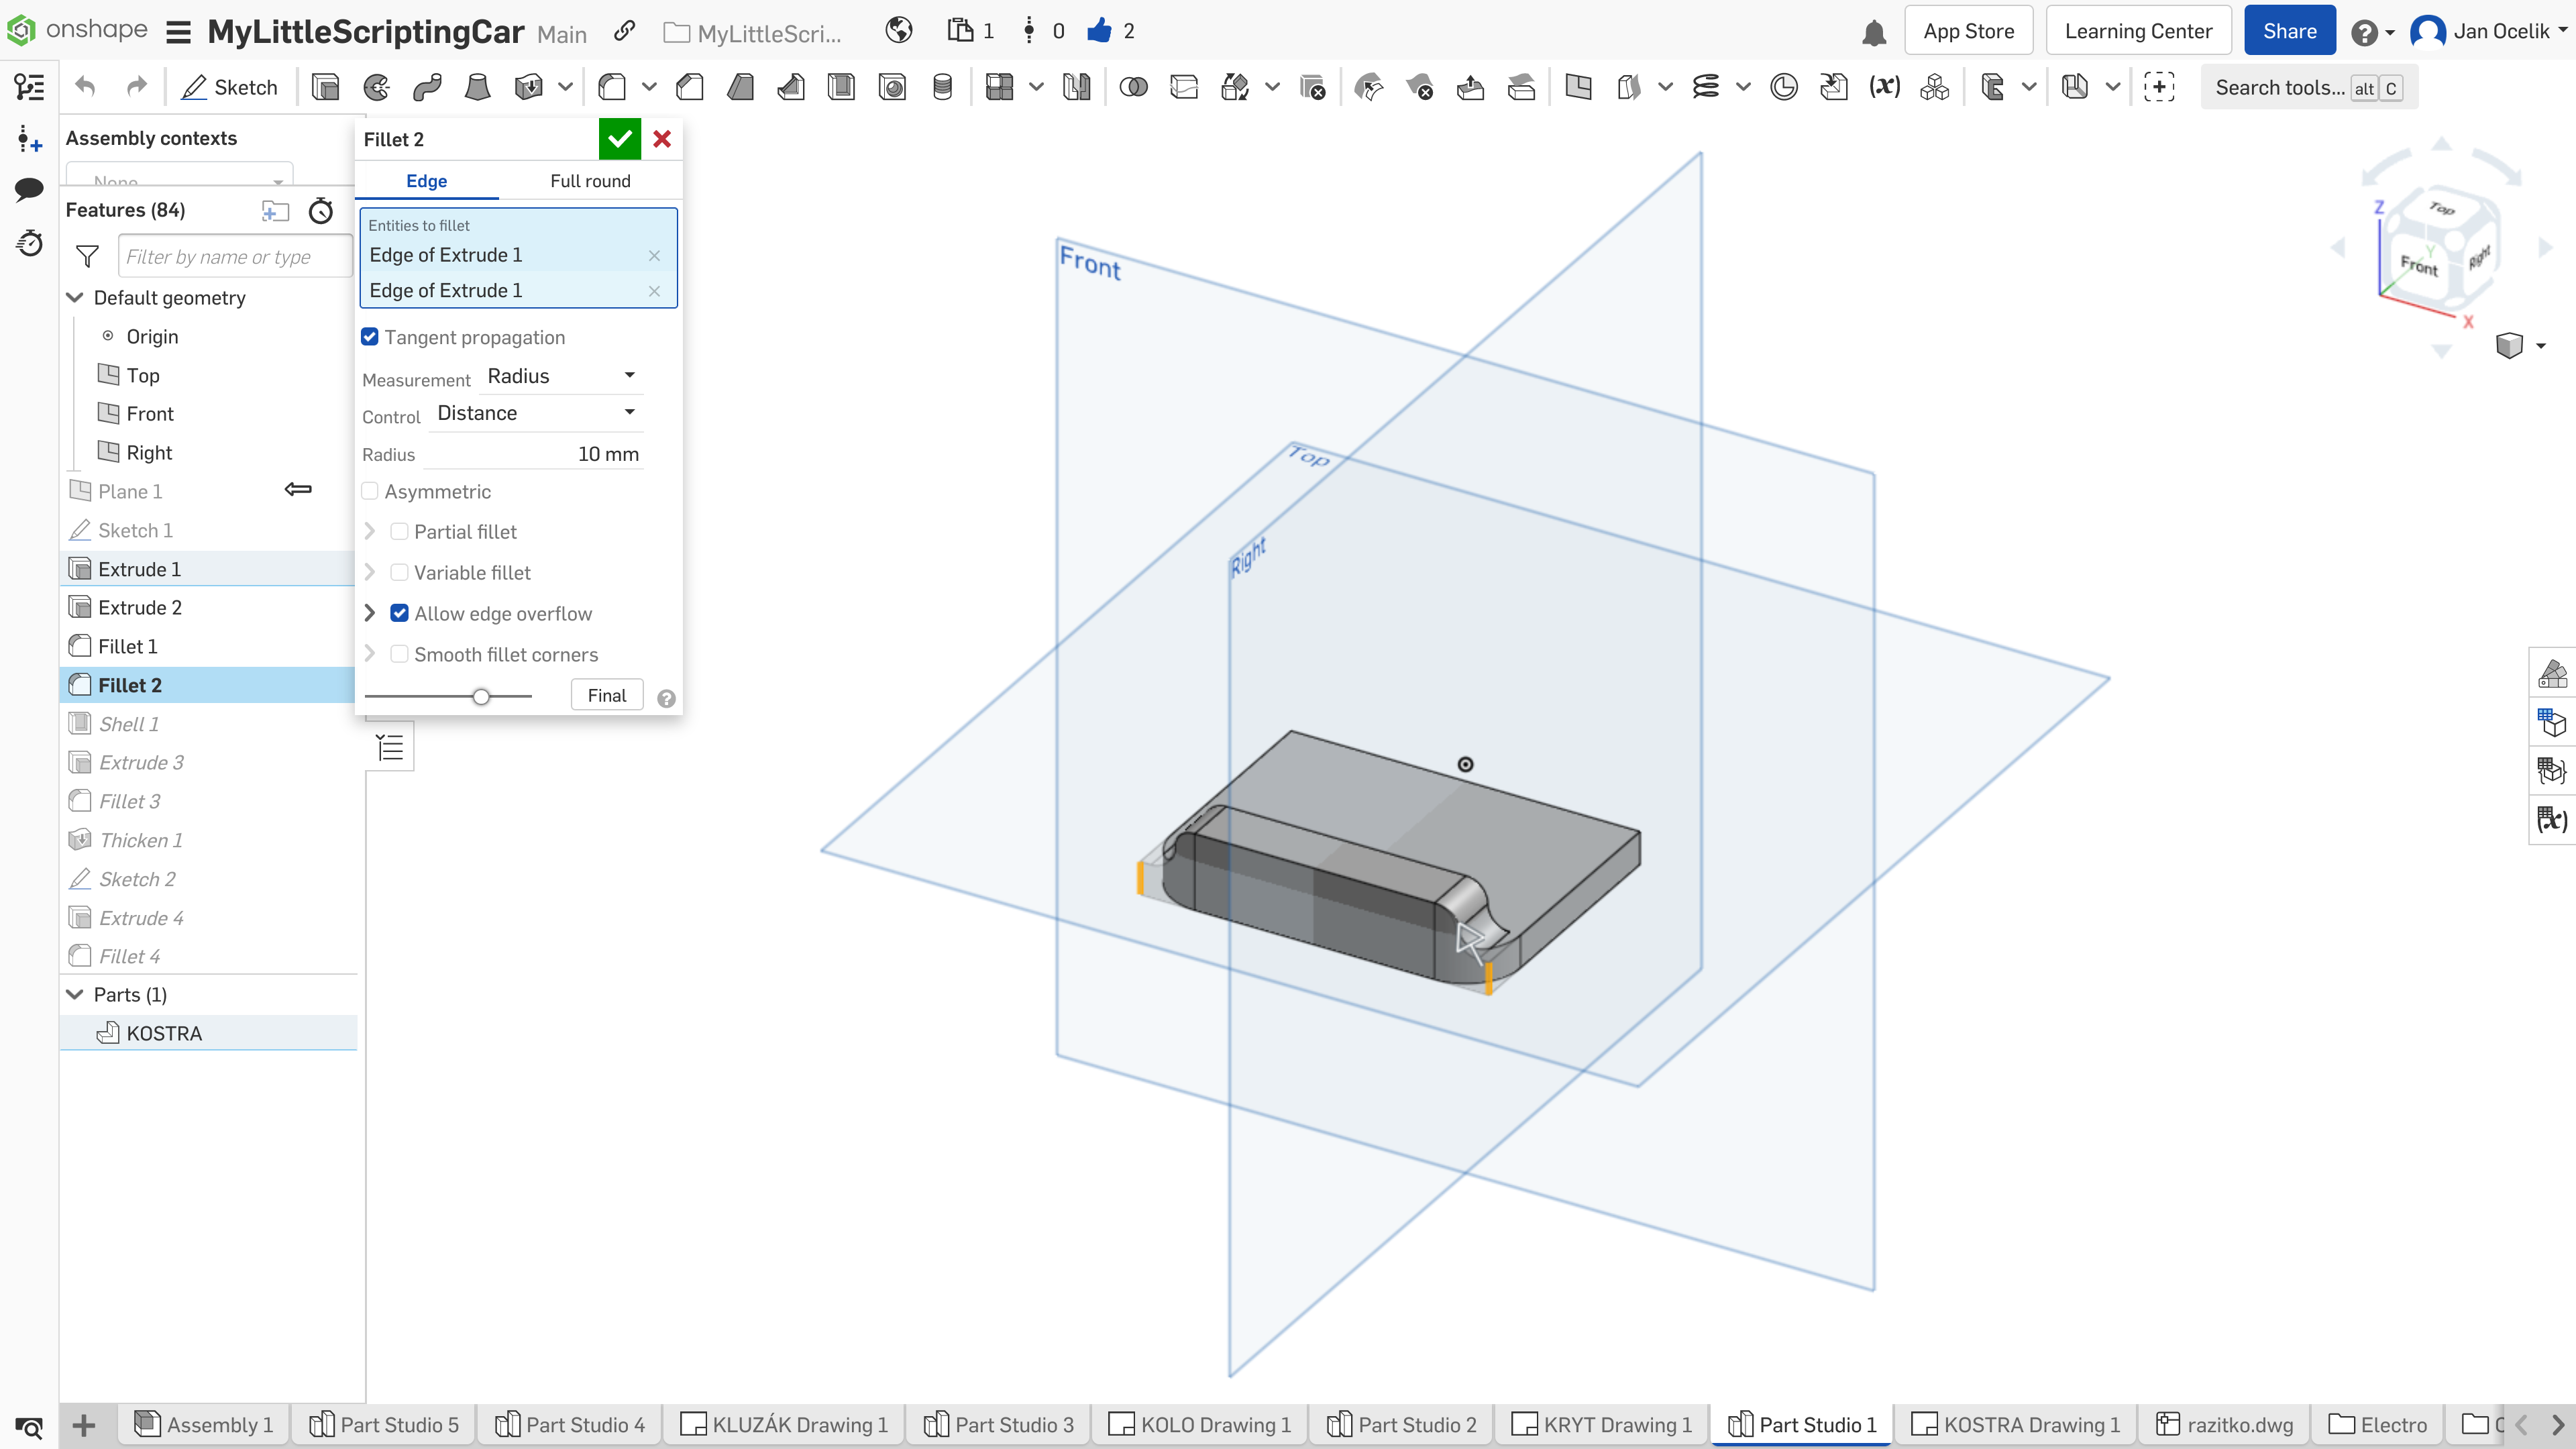
\includegraphics[width=\linewidth]{part_studio}
		\caption{Part Studio}
		\label{fig:part_studio}
	\end{figure}
	
	\subsubsection*{Assembly}
	\paragraph{} Další studio v programu Onshape, Assembly, slouží ke spojování (nebo alespoň aranžování) jednotlivých dílů. K tomuto účelu slouží příkazy, které se opět nechají vyvolat několika způsoby, včetně klepnutím na ikonu v horní liště studia. Další výhodnou funkcí tohoto studia je \textbf{Create Part Studio in context}, což dělá přesně to, co se v názvu píše; vytvoří studio dílu v kontextu se sestavou. Tato funkce může hodně usnadnit vytváření některých dílů.
	
	\begin{figure}[H]
		\centering
		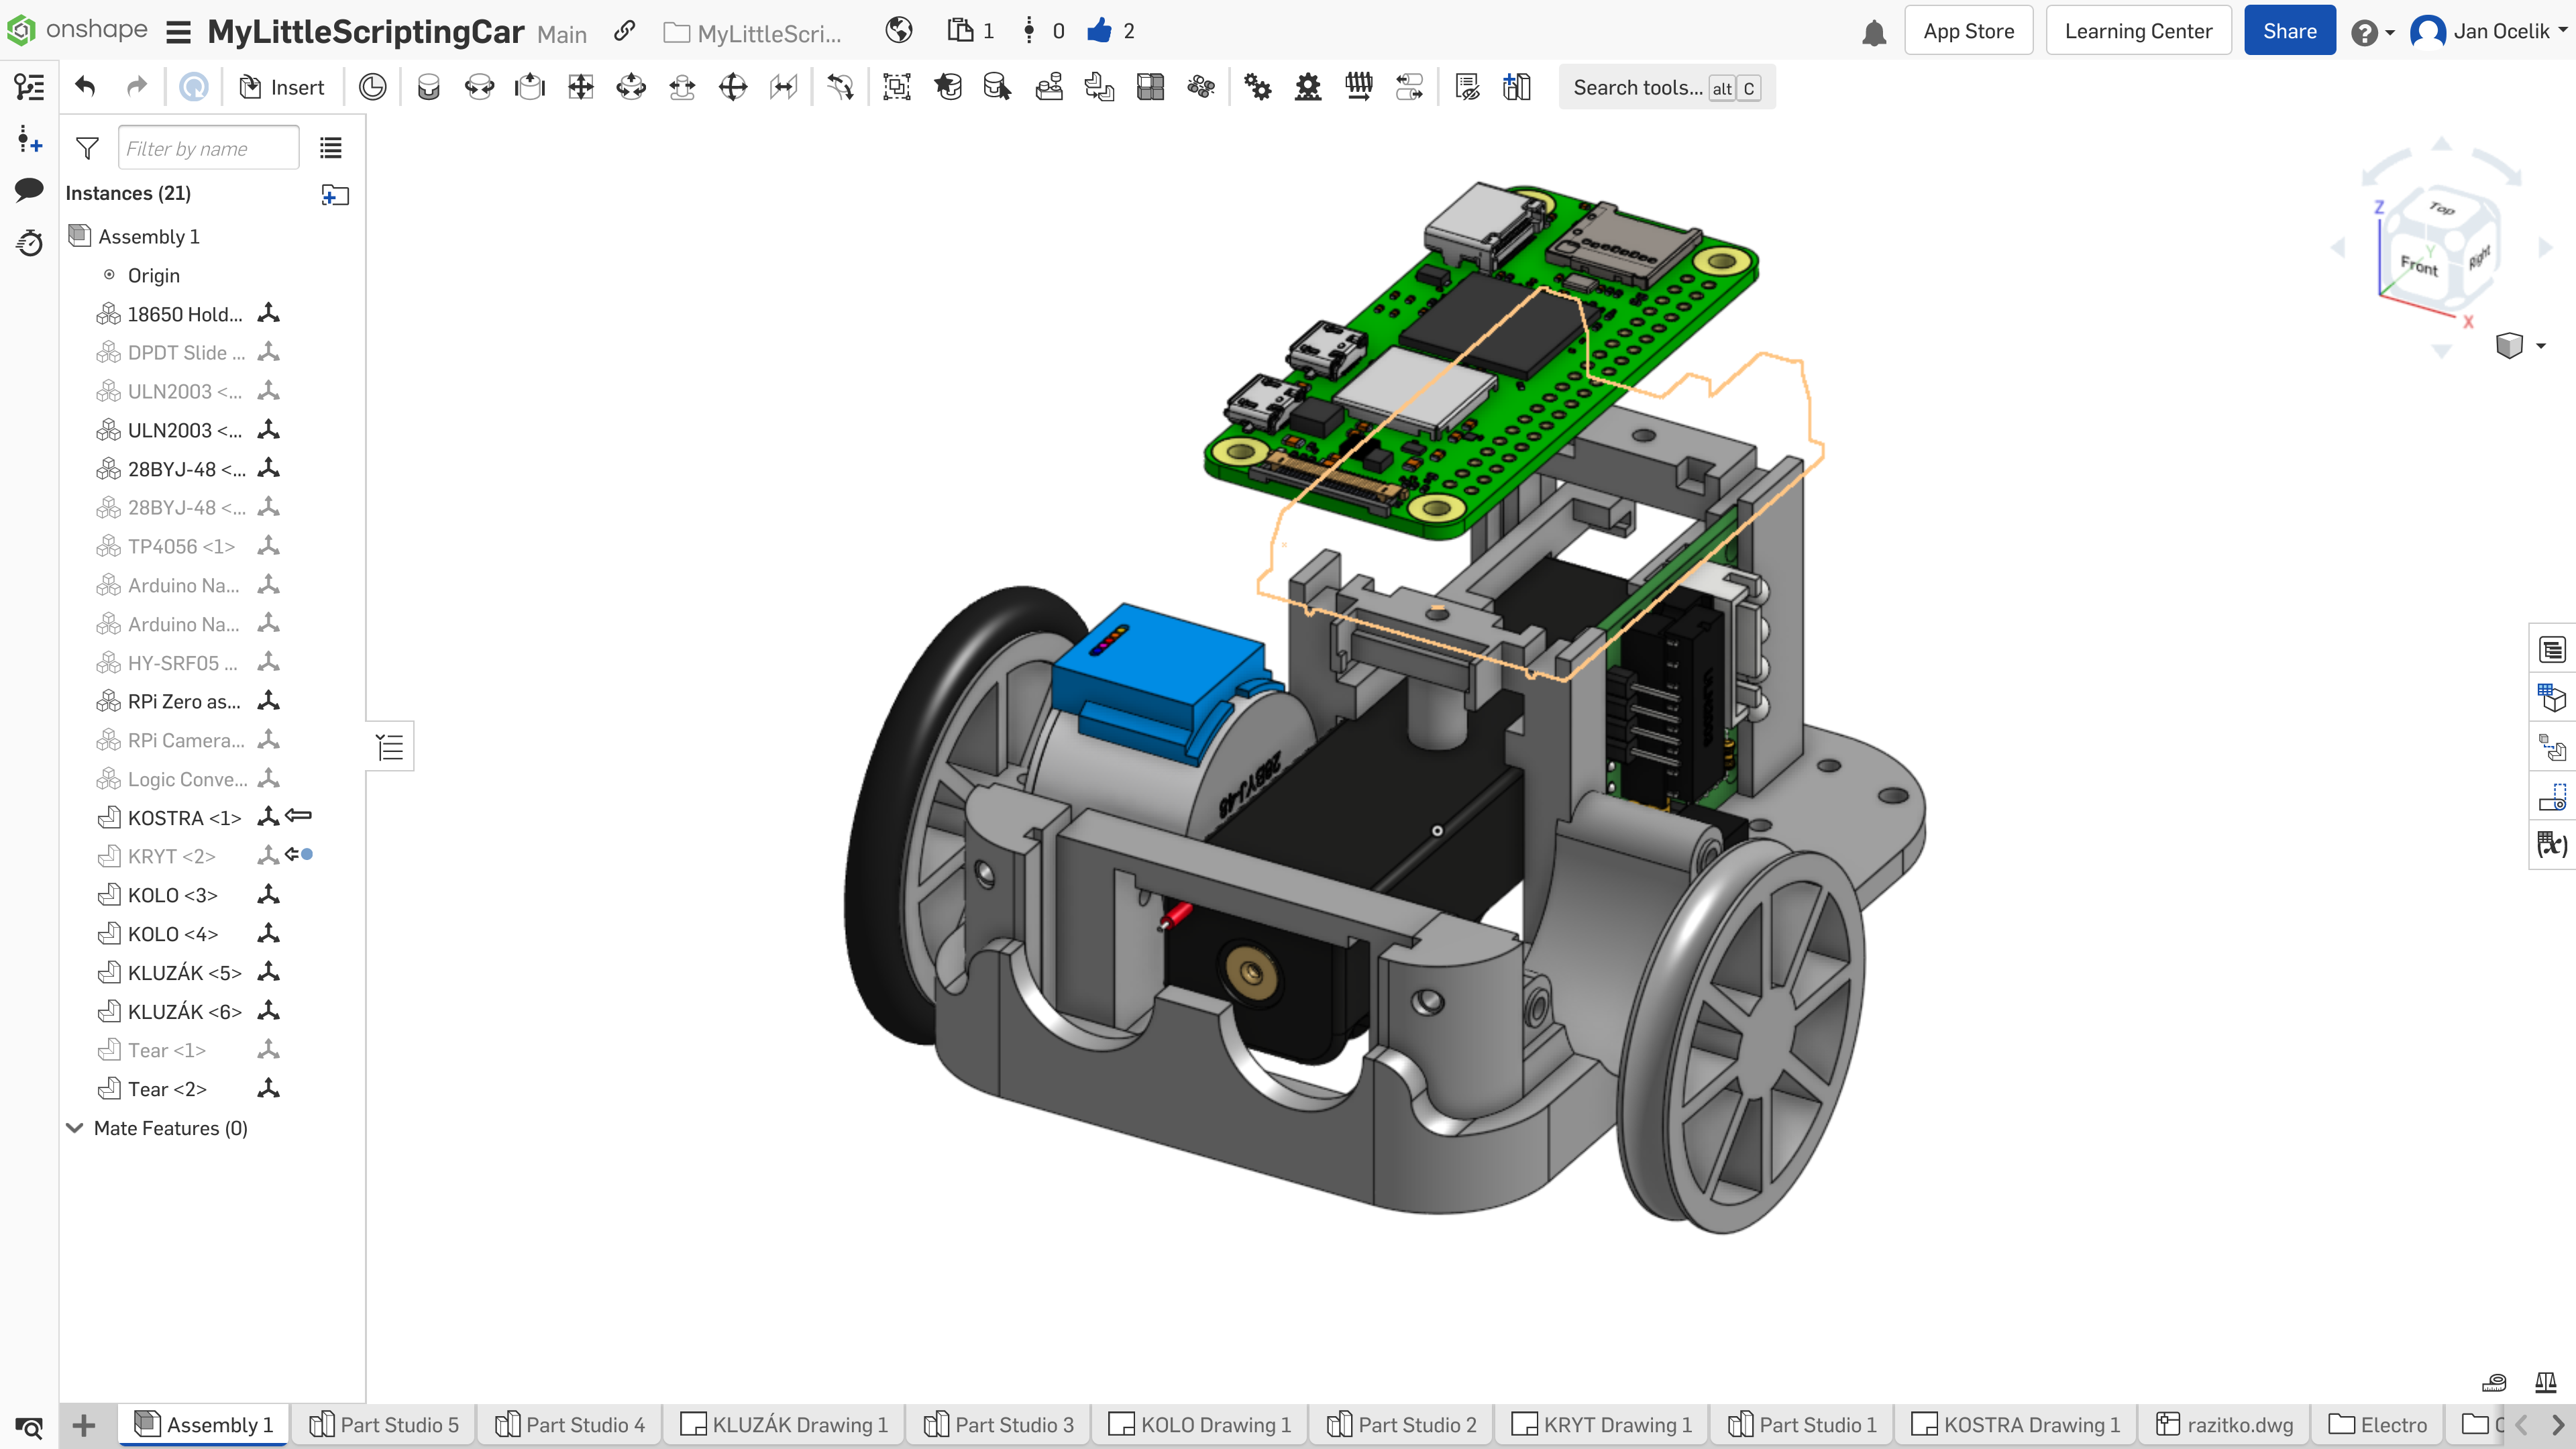
\includegraphics[width=\linewidth]{assembly_studio}
		\caption{Assembly}
		\label{fig:assembly_studio}
	\end{figure}
	
	\subsubsection*{Drawing}
	\paragraph{} Drawing se dá vyvolat jak samostatně, tak rovnou v kontextu s daným dílem a to jak z Part Stuido, tak z Assembly. Uživateli stačí, kdy v seznamu dílů vybere danou položku a přes kontextové menu vybere možnost \textbf{Create Drawing of...}. Výkres se zde upravuje také pomocí příkazů, stejně jako v předešlých studiích. \textbf{Drawing} studio umožňuje také globální nastavení kót, písma, čar atd.
	
	\begin{figure}[H]
		\centering
		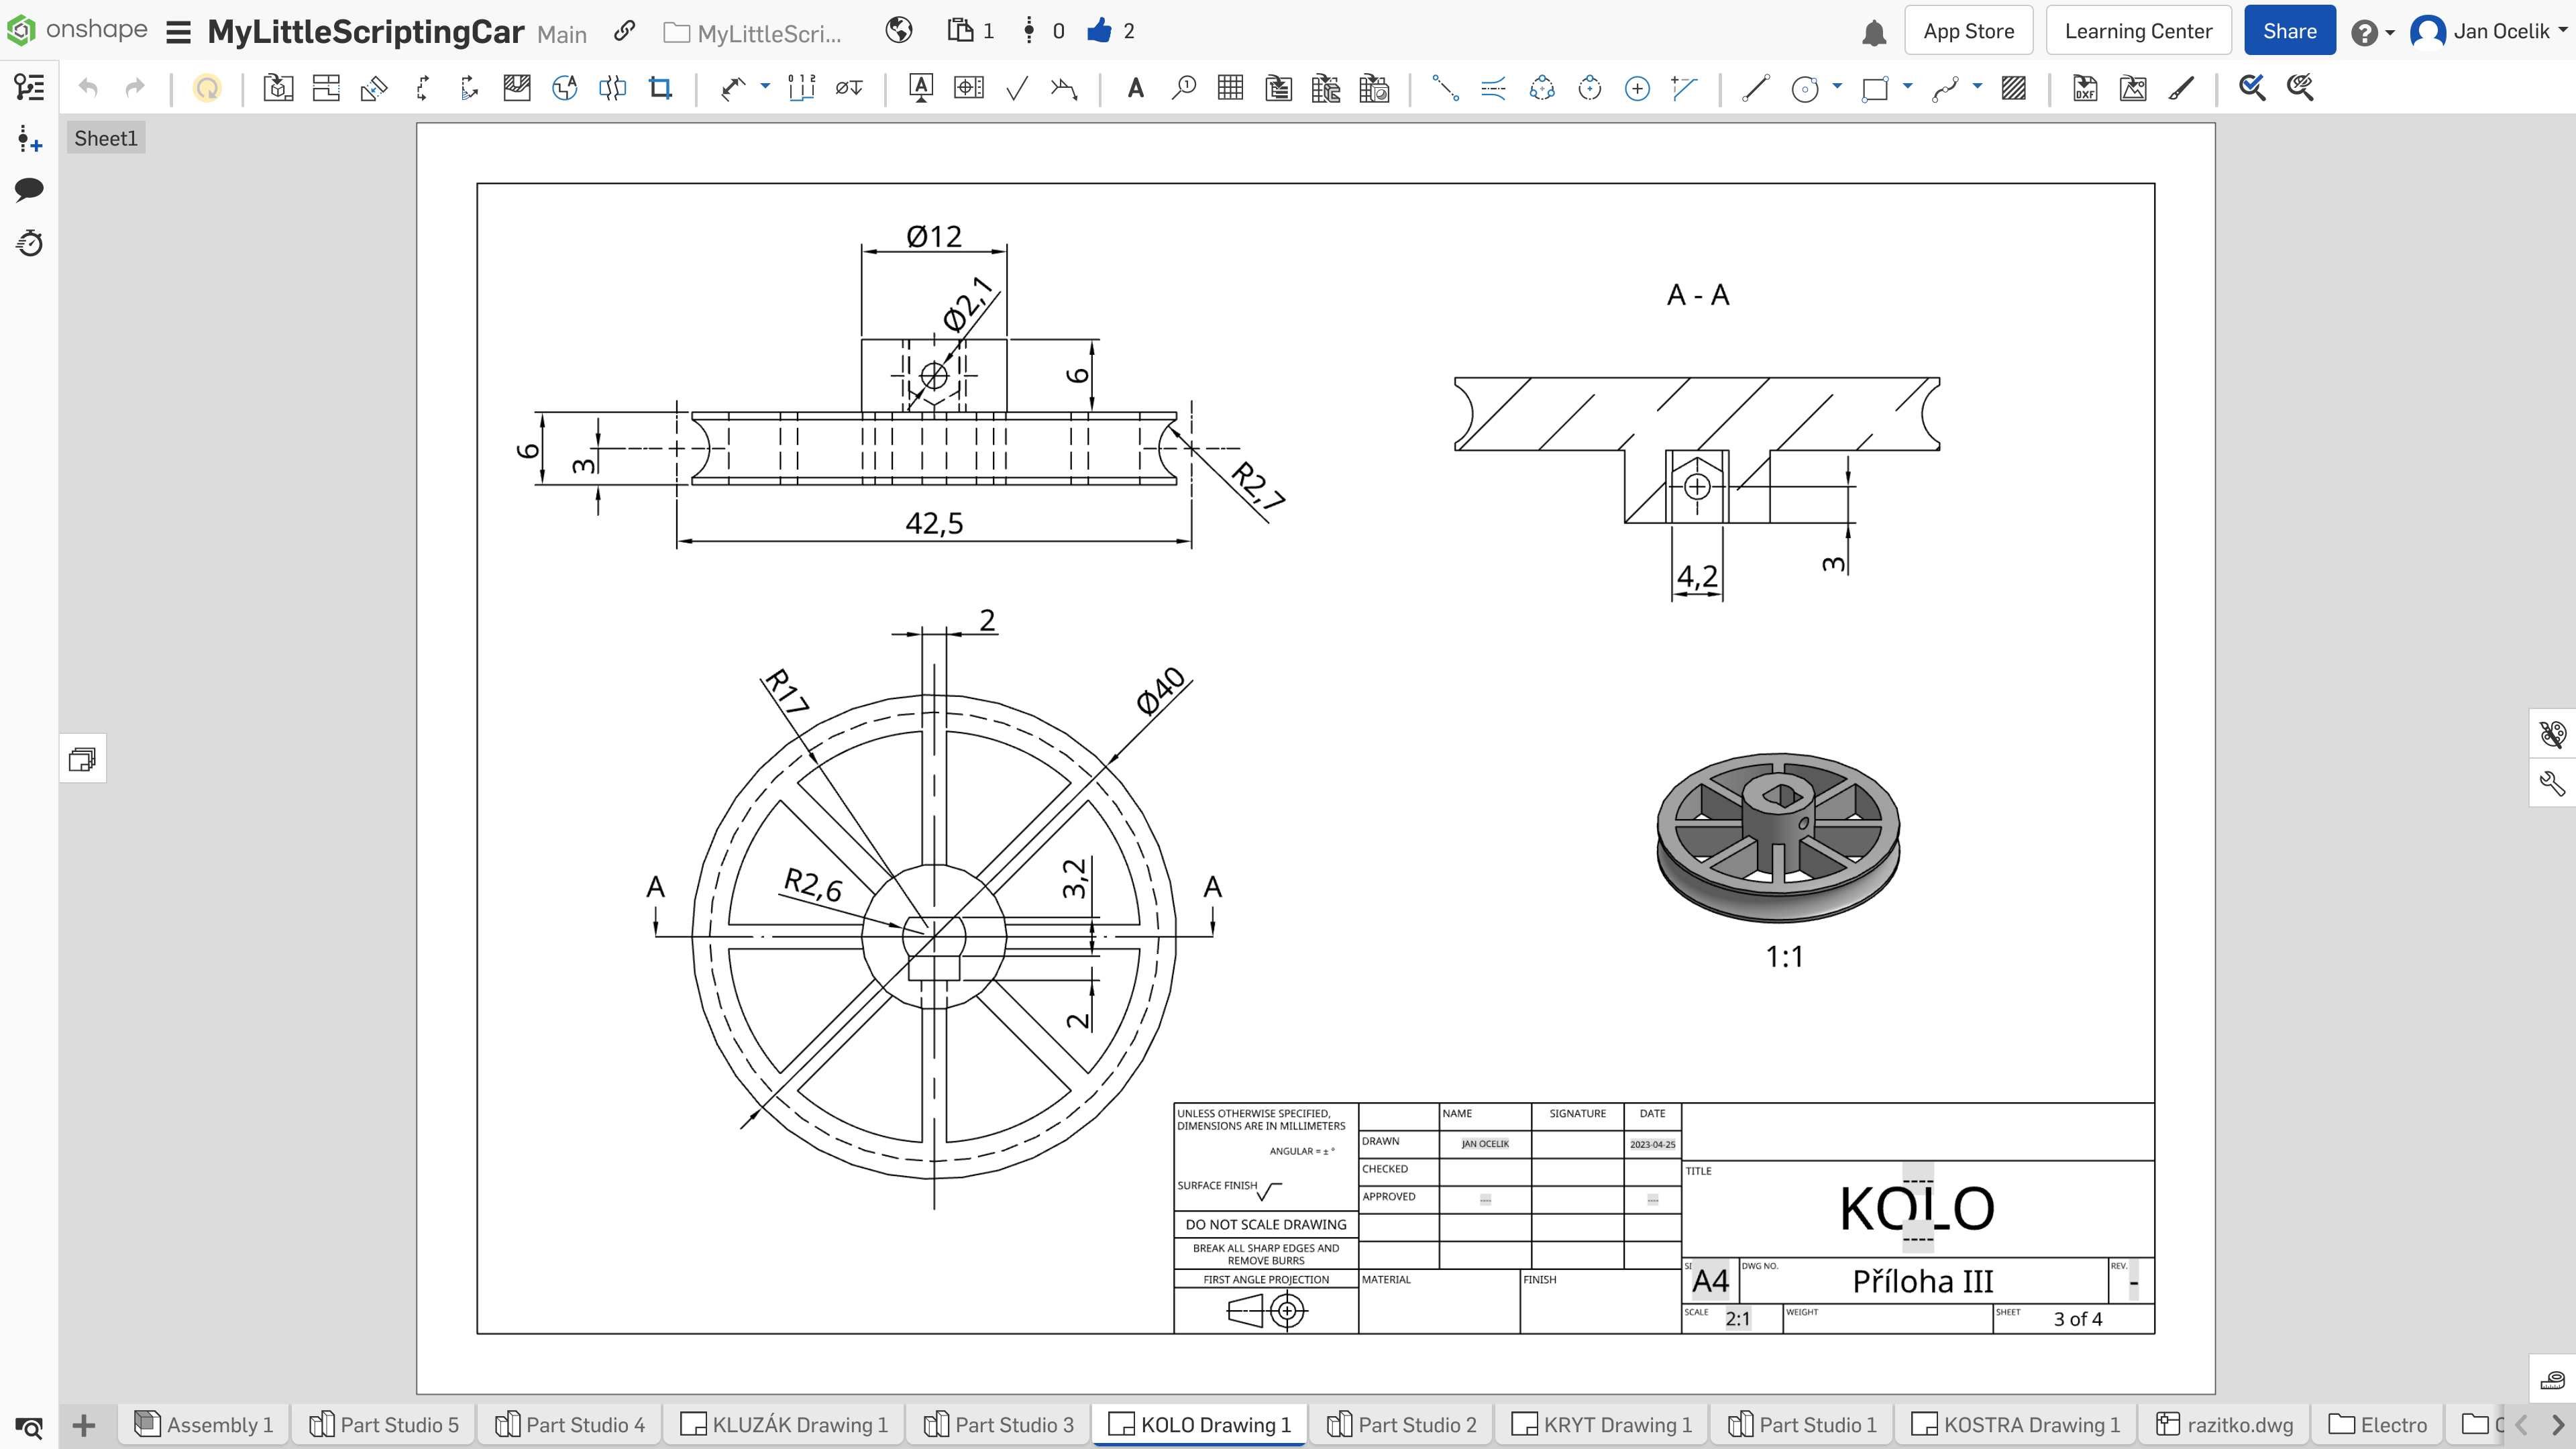
\includegraphics[width=\linewidth]{drawing_studio}
		\caption{Drawing}
		\label{fig:drawing_studio}
	\end{figure}
	
	\subsubsection{Code OSS/VS Code}
	
	\begin{figure}[H]
		\centering
		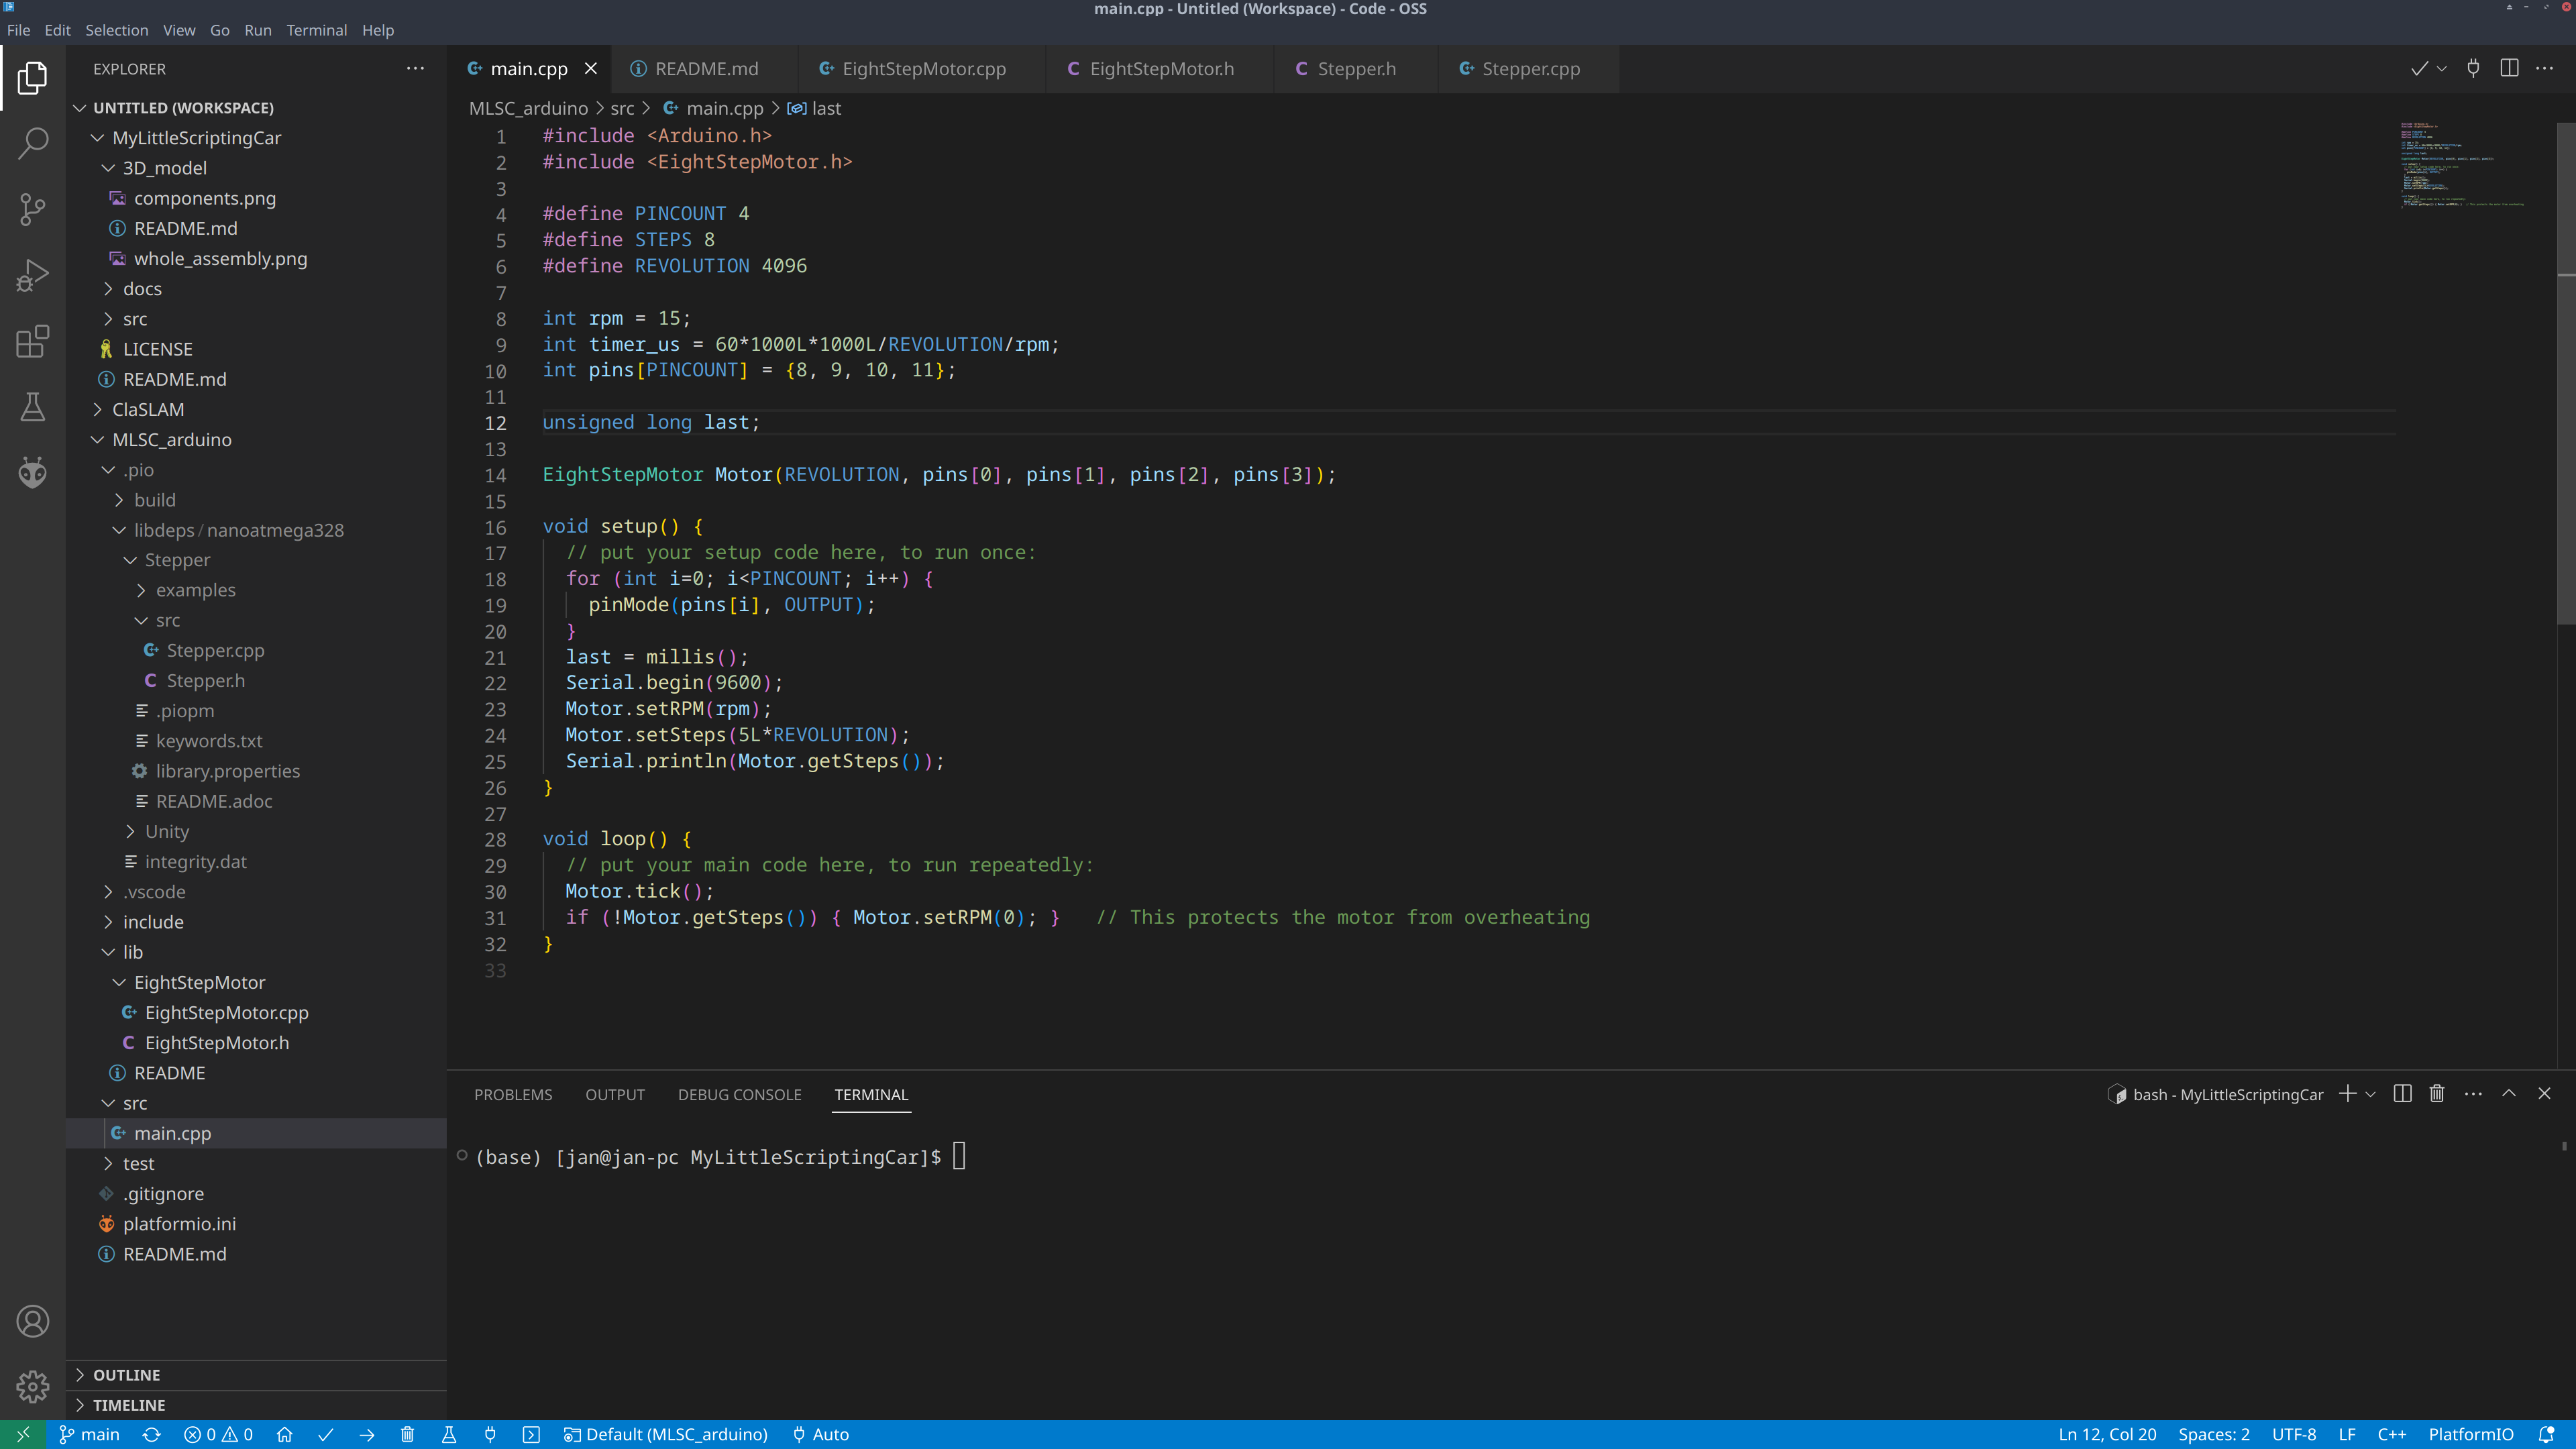
\includegraphics[width=\linewidth]{code_oss}
		\caption{Code OSS}
		\label{fig:code_oss}
	\end{figure}
	
	\paragraph{} Code OSS je opensource IDE vyvíjené firmou Microsoft. Vzniklo jako konkurent programu Atom, který se nyní již nevyvíjí. Stal se tak oblíbeným hlavně díky podpoře obrovského množství programovacích i značkovacích jazyků (např. python, c++, java, xml, html). Má také velice intuitivní ovládání a šikovně zvolenou paletu barev.
	
	\paragraph{} Code OSS a Visual Studio Code jsou téměř identické programy, jediným pozorovatelným rozdílem je absence některých rozšíření v \uv{marketplace} v Code OSS (i to se dá ale snadno opravit).
	
	\subsubsection*{PlatformIO}
	\paragraph{} Platformio je rozšíření do VS Code umožňující překlad C++ kódu a následný upload do předdefinovaných jednočipů (např. atmega328). Je to šikovný kus softwaru s několika užitečnými funkcemi navíc, jako např. automatická detekce zařízení, seznam dostupných knihoven, snadná instalace a integrace daných knihoven do projeků.
	
	\begin{figure}[H]
		\centering
		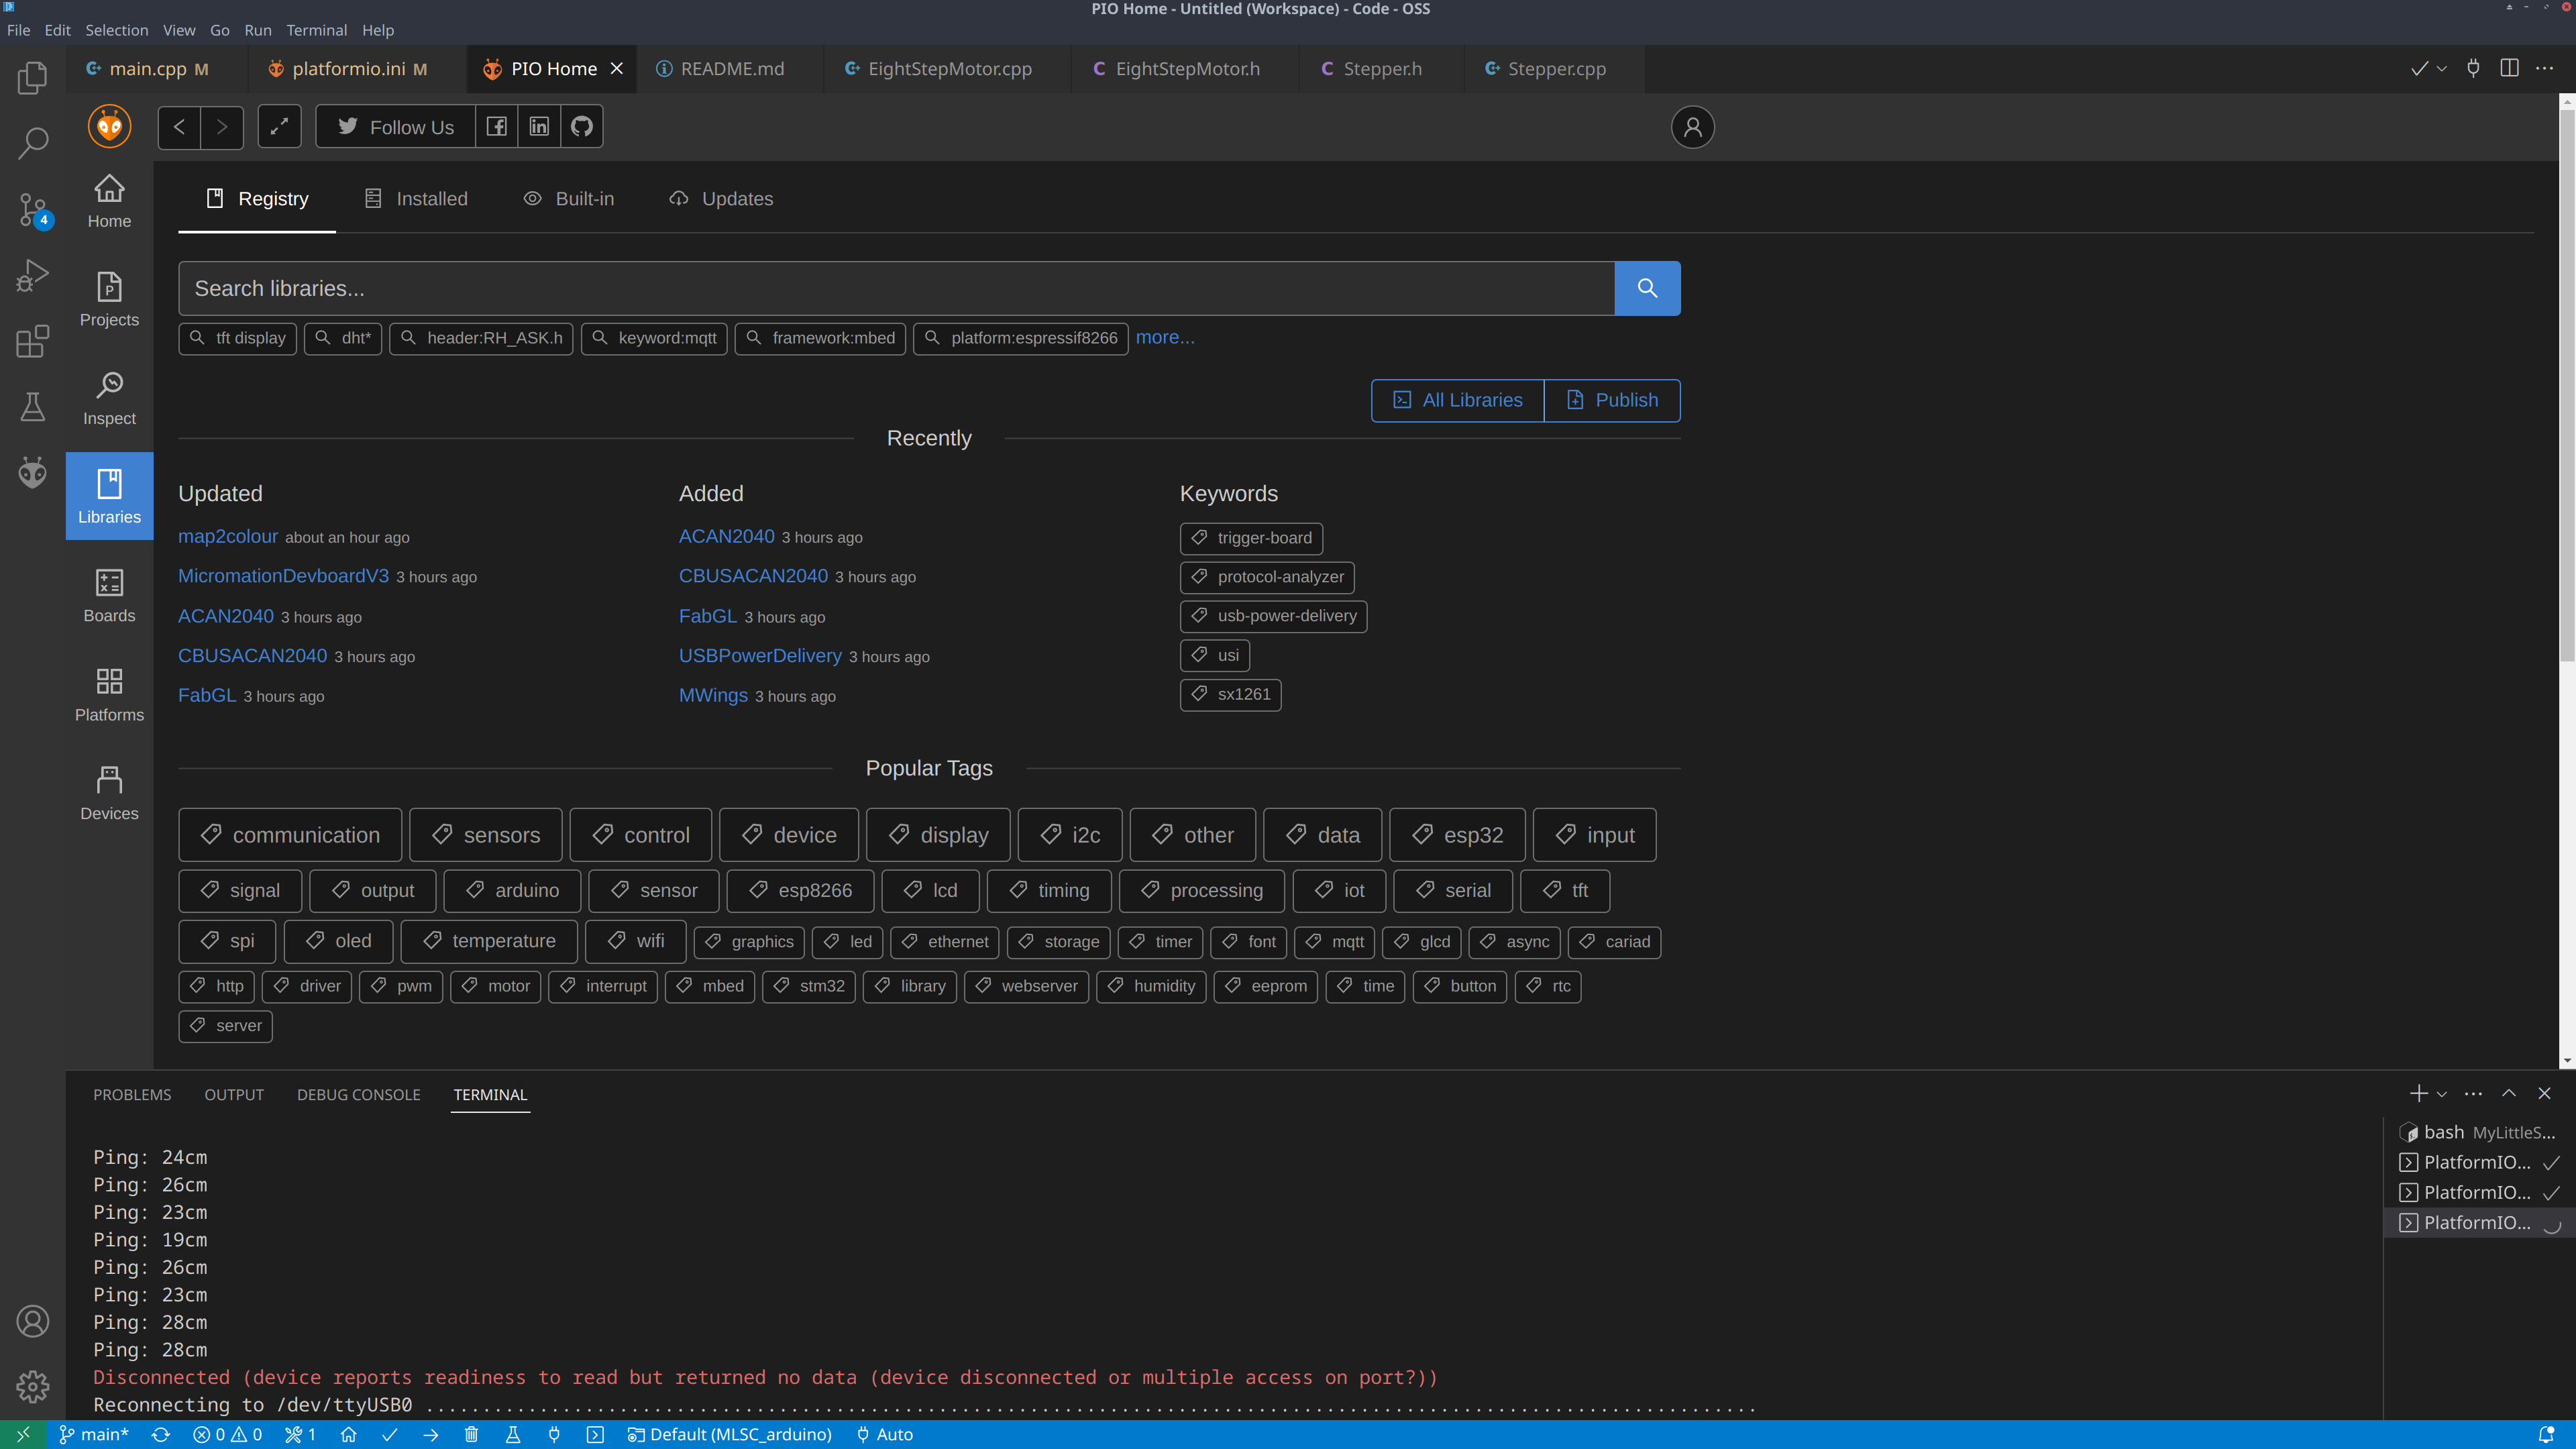
\includegraphics[width=\linewidth]{platformio}
		\caption{PlatformIO}
		\label{fig:platformio}
	\end{figure}
	
	% Výrobní technologie
	\newpage
	\subsection{Výrobní technologie}
	\subsubsection{3D tisk}
	\paragraph{} 3D tisk je moderní technologie, která umožňuje vytvářet fyzické objekty ze 3D digitálních modelů. Tento proces začíná vytvořením digitálního modelu pomocí počítačového softwaru. Poté je tento digitální model převeden do formátu, který je kompatibilní s 3D tiskárnou. V~průběhu tiskového procesu se materiál, obvykle termoplastického typu, zahřívá a aplikuje na specifická místa v souladu s digitálním modelem. Tento postup se opakuje vrstva po vrstvě, dokud není celý objekt hotov.
	
	\paragraph{} 3D tisk má mnoho výhod. Například umožňuje rychlé prototypování a výrobu malých sérií komplexních geometrických objektů. To se stává velmi užitečné v oblasti průmyslové výroby, kde může být vytvoření prototypu značně nákladné a časově náročné. Díky 3D tisku se náklady na výrobu mohou snížit a doba výroby může být zkrácena.
	
	\paragraph{} V posledních letech se cena 3D tiskáren snížila a uživatelé si mohou tisknout vlastní návrhy přímo z domova. Tato technologie také umožňuje vytvářet přizpůsobené a jedinečné předměty, což je velmi užitečné pro řadu různých aplikací, včetně medicíny, průmyslu a uměleckých oborů.
	
	\paragraph{} Díky jednoduchosti použití a možnosti tvorby téměř jakýchkoli tvarů je ideální volbou k~výrobě kostry programovatelného auta.
	
	\begin{figure}[H]
		\centering
		\includegraphics[width=\linewidth]{tisk_kostra_kryt}
		\caption{Vytištěný model kostry, kol a kluzáků auta (vlevo) -- Tisk modelu krytu (vpravo)}
		\label{fig:tisk_kostra_kryt}
	\end{figure}

	% Vybrané komponenty (moduly)
	\newpage
	\section{Popis konstrukce a vybrané moduly}
	\subsection{Vybrané moduly}
	
	\paragraph{} Pro ovládání motorů bylo nutné vybrat \uv{řídící jednotku}. Pro tento účel se nejen kvůli rozměrům jevila jako jasná volba Arduino Nano, ale kvůli ceně bylo lepší sáhnout po dostupnějším klonu: \textbf{\textit{Robotdyn Arduino Nano V3}}.
	Piny na arduinu jsou přístupné pouze ze spodní strany desky, což je vzhledem k jeho umístění v robotovi dosti nešikovné. Elegantním řešením problému je takzvaný terminál, který piny zpřístupní z boků.
	
	\paragraph{} Kvůli předpokládanému univerzálnímu využití robota bylo nutné zvolit také vhodný pohon. Tím se ukázaly být krokové motory. K motorům jsou potřeba také řadiče a to kvůli velkým proudům, které mohou motory procházet.
	Aby mohl být robot alespoň částečně autonomní, je téměř nutností přidat nějaké vstupní periferie, které poslouží k získávání zpětné vazby k řízení, jako například: \textbf{\textit{Ultrazvukový měřič vzdálenosti HY-SRF05}}.
	
	\paragraph{} Pro správné fungování robota bylo nutné zvolit vhodné napájení. U autonomního zařízení je jasnou volbou nabíjecí baterie a díky své popularitě a rozšíření je nejlepší možností \textbf{\textit{Li-ion baterie 18650}} v kombinaci s dobíjecím modulem \textbf{\textit{M 401A}}.
	Na baterii je také nutné vybrat vhodný držák a vzhledem k jejímu umístění je potřeba zvolit takový, který baterii udrží ve správné pozici i při hrubším zacházení s robotem.
	Je také nutné mít možnost robota nějak vypnout/odpojit (přerušit obvod), v ideálním případě napájecí obvod kompletně izolovat. Proto je dobré zvolit dvoucestný přepínač, například \textit{\textbf{posuvný dvojitý přepínač}}.
	
	\paragraph{} \textbf{\textit{Raspberry Pi Zero 2 w}} je vhodným modulem pro rozšíření funkcí robota, který se propojí s Arduinem (řídícím modulem) pomocí asynchronní sériové linky a umožní tak rychlejší zpracování údajů získaných z dalších rozšiřujících modulů, například z \textbf{\textit{Raspberry Pi Camera 2 NoIR}}. Protože Raspberry a Arduino pracují na různých hladinách napětí, je potřeba pro bezpečné propojení a komunikaci mezi těmito moduly použít \textit{\textbf{převodník logických hodnot}}.
	
	\begin{figure}[H]
		\centering
		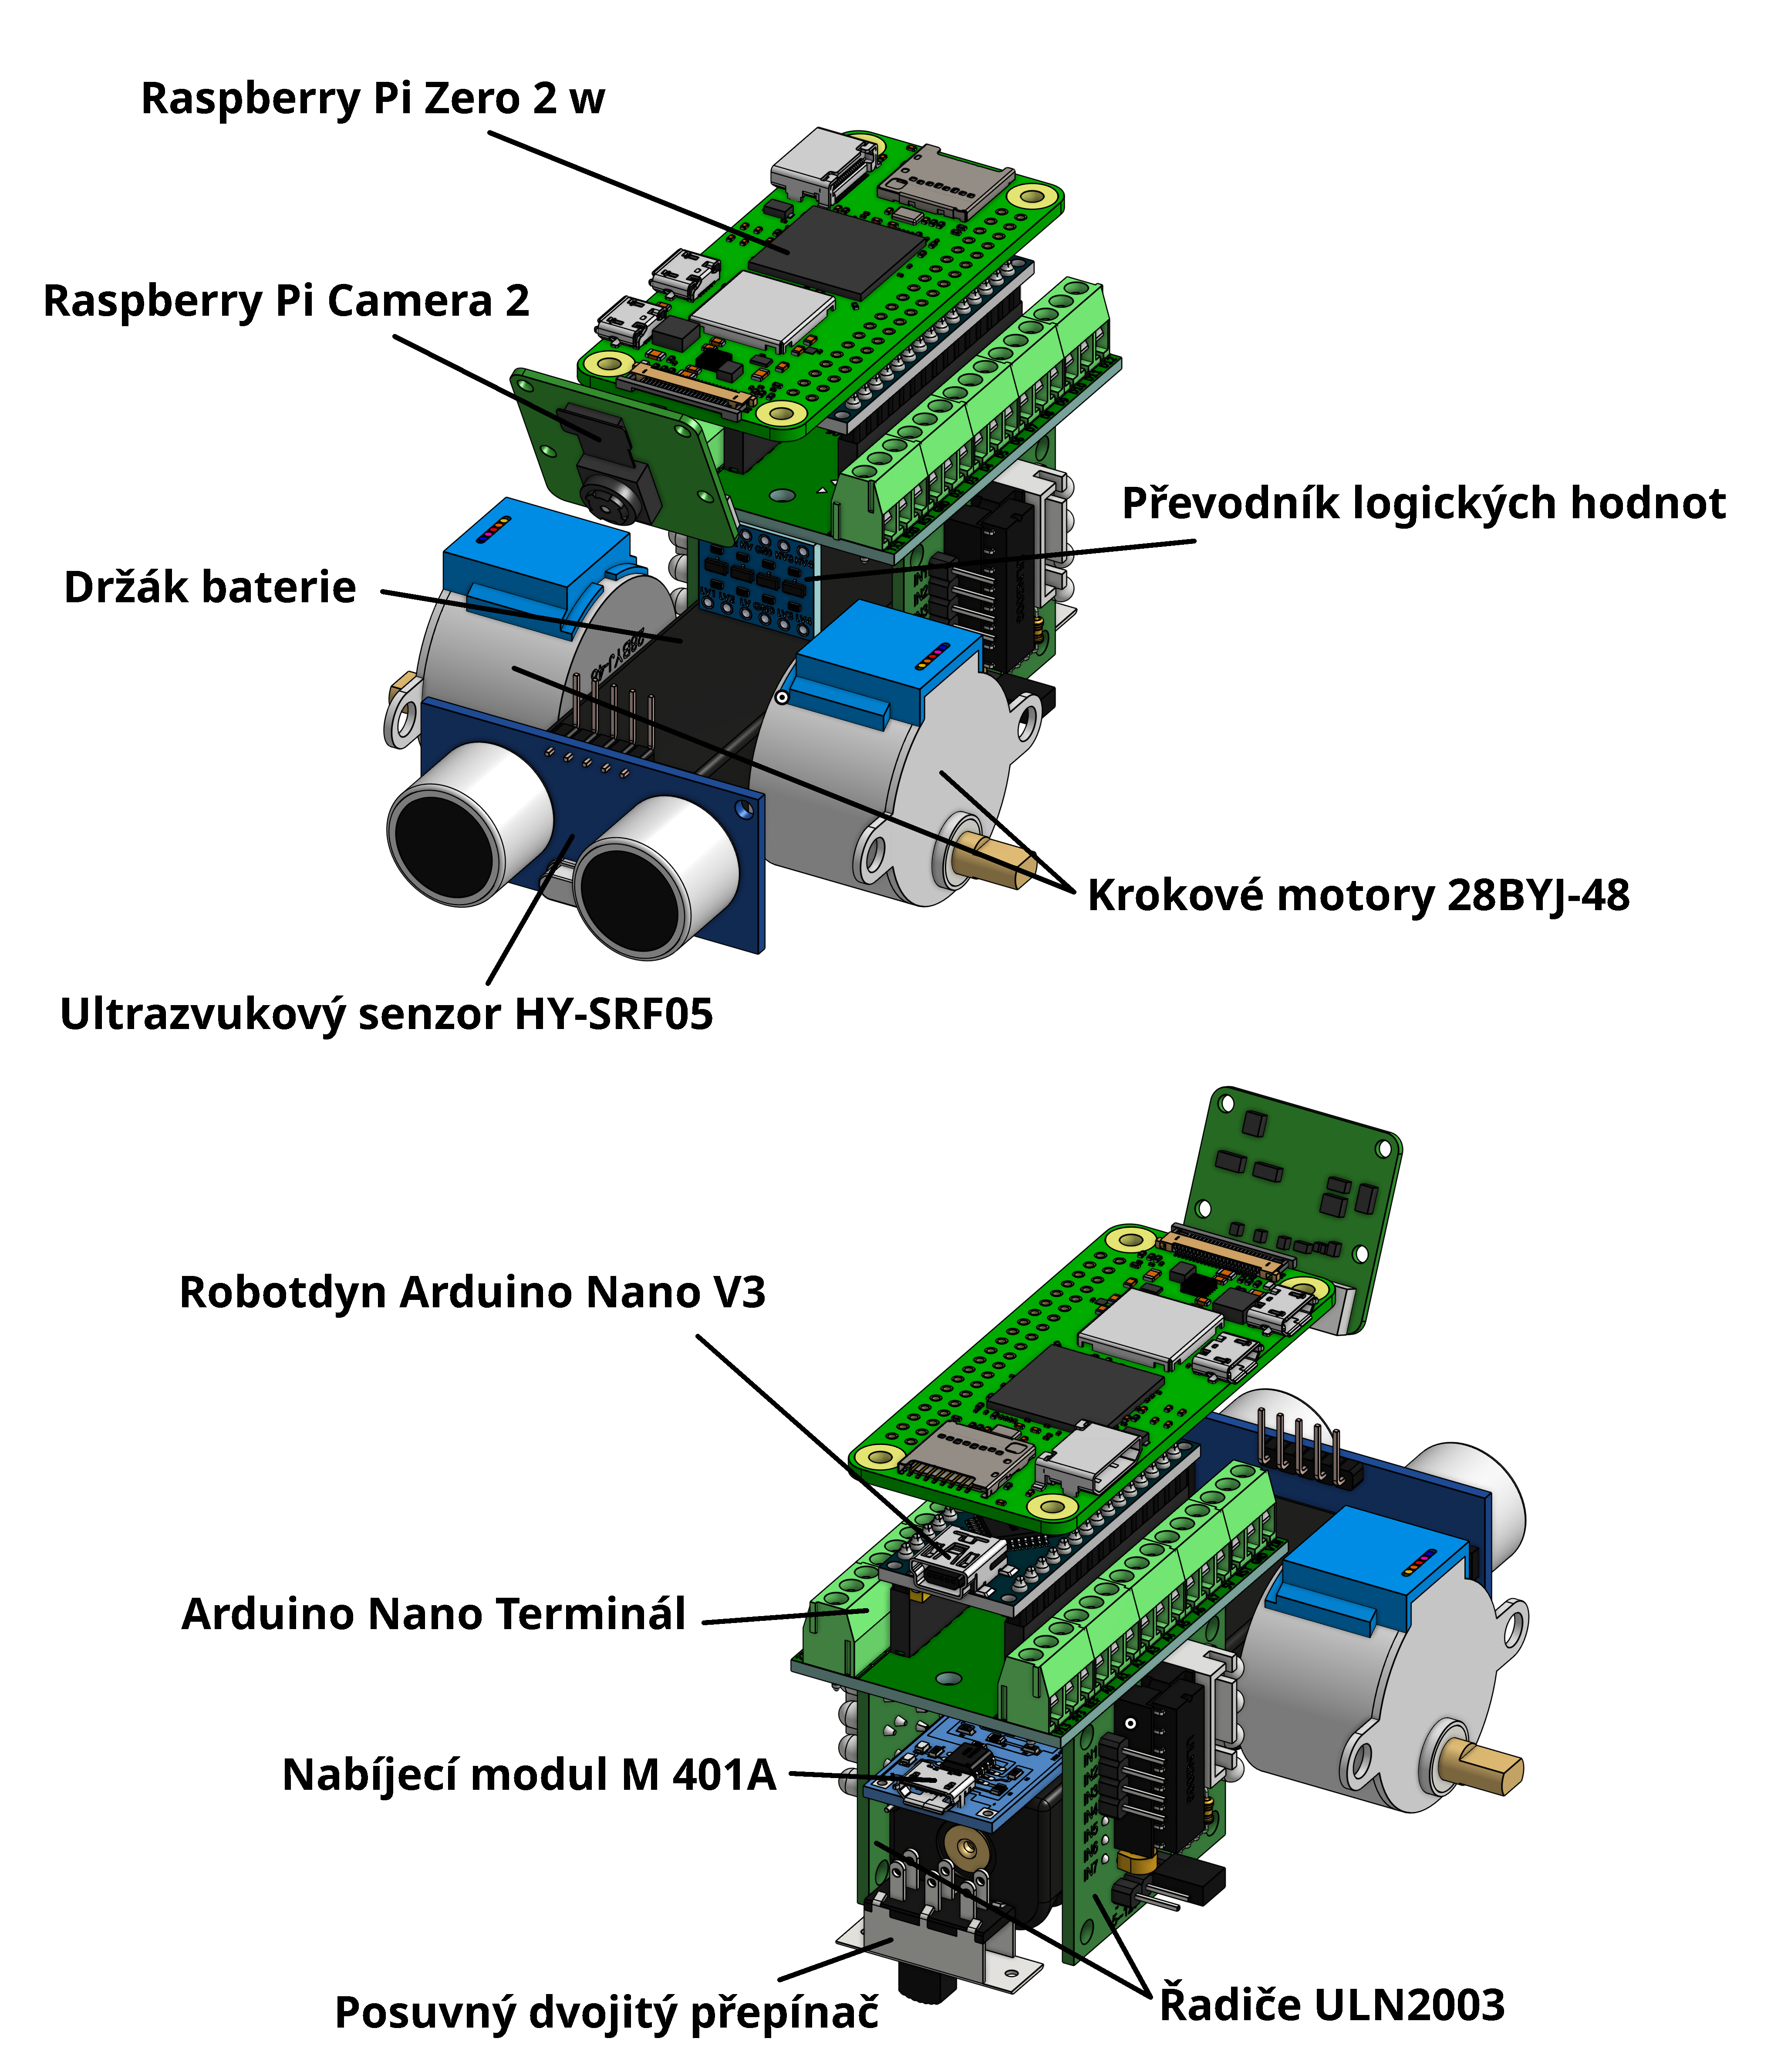
\includegraphics[width=\linewidth]{moduly}
		\caption{Umístění modulů v robotovi}
		\label{fig:moduly}
	\end{figure}
	\newpage	
	\subsection{Konstrukce}
	\paragraph{} Cílem této práce bylo navrhnout kostru programovatelného auta tak, aby bylo co nejkompaktnější a zároveň aby se zachovala snadná přístupnost ke všem integrovaným modulům.
	
	Kostra je navržena tak, aby většina modulů mohla být nainstalována pouhým zasunutím do drážek a pomocí gravitace, zacvaknutím, nebo překrytím jiným modulem. Díky tomu bylo použito co nejméně šroubových spojů.
	
	Krokové motory bylo třeba pevně ukotvit usazením do výřezů, které kopíruje tvar jejich těl, a zajištěním samořeznými šrouby.
	
	Ultrazvukový senzor je zasunut do drážky, která jej těsně obklopuje ze tří stran. Zamezí se tím nežádoucím vibracím senzoru při pohybu robota.
	
	Držák baterie je kvůli usnadnění výměny baterie umístěn na spodní straně tak, aby baterie byla přístupná bez nutnosti odstraňovat kryt robota. Napájecí obvod, včetně nabíjecího modulu, je snadno přístupný a může tak být v případě potřeby bez problémů vymontován.
	
	Vypínač je umístěn na spodní straně vzadu a ke kostře pevné uchycen samořeznými šrouby, kvůli předpokládanému častému používání.
	
	Arduino je umístěno tak, aby byl snadno přístupný jeho programovací konektor. Pomocí terminálu, do nějž je Arduino zasunuto, byly zpřístupněny všechny jeho piny (svorky). Samotný terminál je ukotven ke kostře samořeznými šrouby.
	
	Vzhledem k vysoké kompaktnosti robota byly použity pouze dva krokové motory, tedy navržené auto má pouze dvě kola. Pro zajištění stability auta je nutné mít alespoň tři opěrné body (zde dvě kola a jeden kluzák). Kvůli umístění vypínače uprostřed robota bylo nutné zvýšit počet dodatečných opěrných bodů (kluzáků) na dva a umístit je po stranách vypínače.
	
	Aby se zabránilo prokluzování kol na osách krokových motorů, jsou navržená kola vybavena integrovanou matičkou a šroubkem M2, které pomocí tření zabrání sklouznutí kola z osy.
	
	Pro zvýšení přilnavosti kol k podkladu při pohybu robota byla použita toroidová těsnění (průměr 42mm/5,5mm), která jsou usazena v drážce na kolech.
	
	Základ robota obsahuje pouze Arduino a moduly, které zajišťují základní funkce: pohyb, napájení a sběr dat ze vstupní periferie (Ultrazvukového senzoru).
	
	\begin{figure}[H]
		\centering
		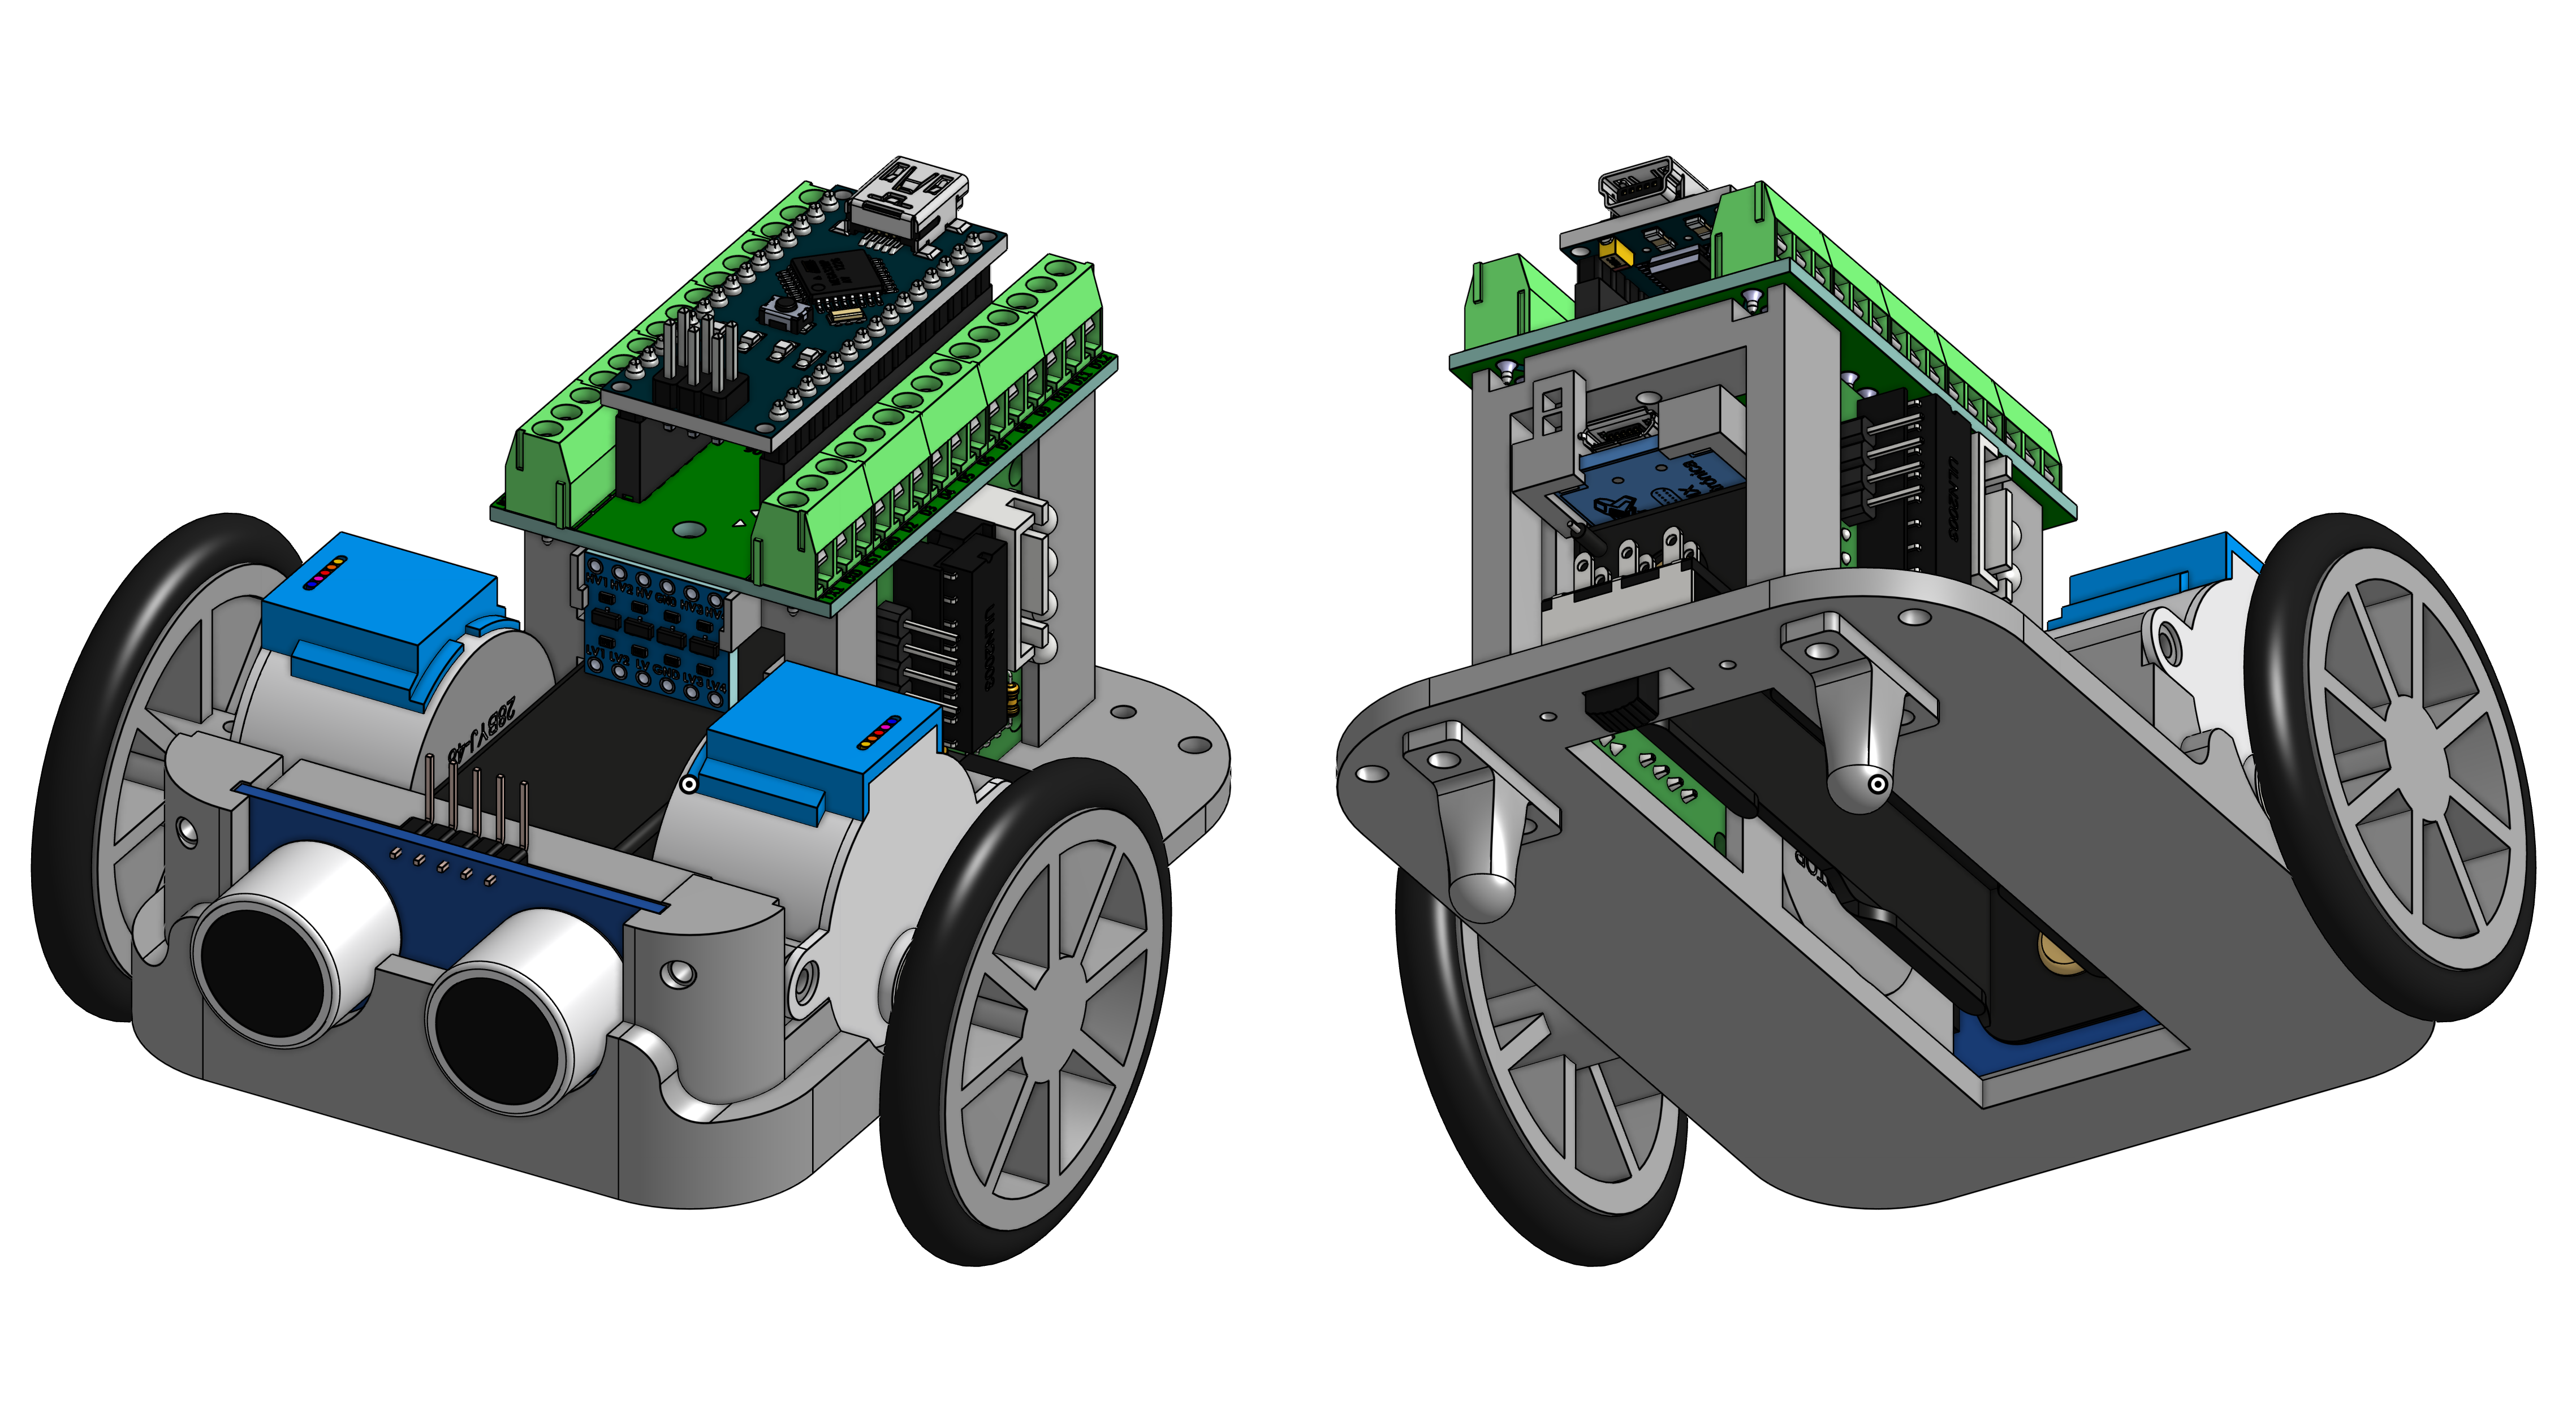
\includegraphics[width=\linewidth]{moduly_kostra}
		\caption{Umístění modulů na kostře auta}
		\label{fig:moduly_kostra}
	\end{figure}
	
	Na zádech robota je provizorně umístěna kamera a Raspberry Pi, které slouží v této práci pouze k demonstraci řízení robota posíláním příkazů přes sériovou linku Arduinu a pomocí dat získaných z ultrazvukového senzoru a kamery připojené přímo do Raspberry Pi. Tímto propojením se, obrazně řečeno, z Arduina stává \uv{mícha}, která předává příkazy z \uv{mozku} (Raspberry Pi) do periferií.
	
	\begin{figure}[H]
		\centering
		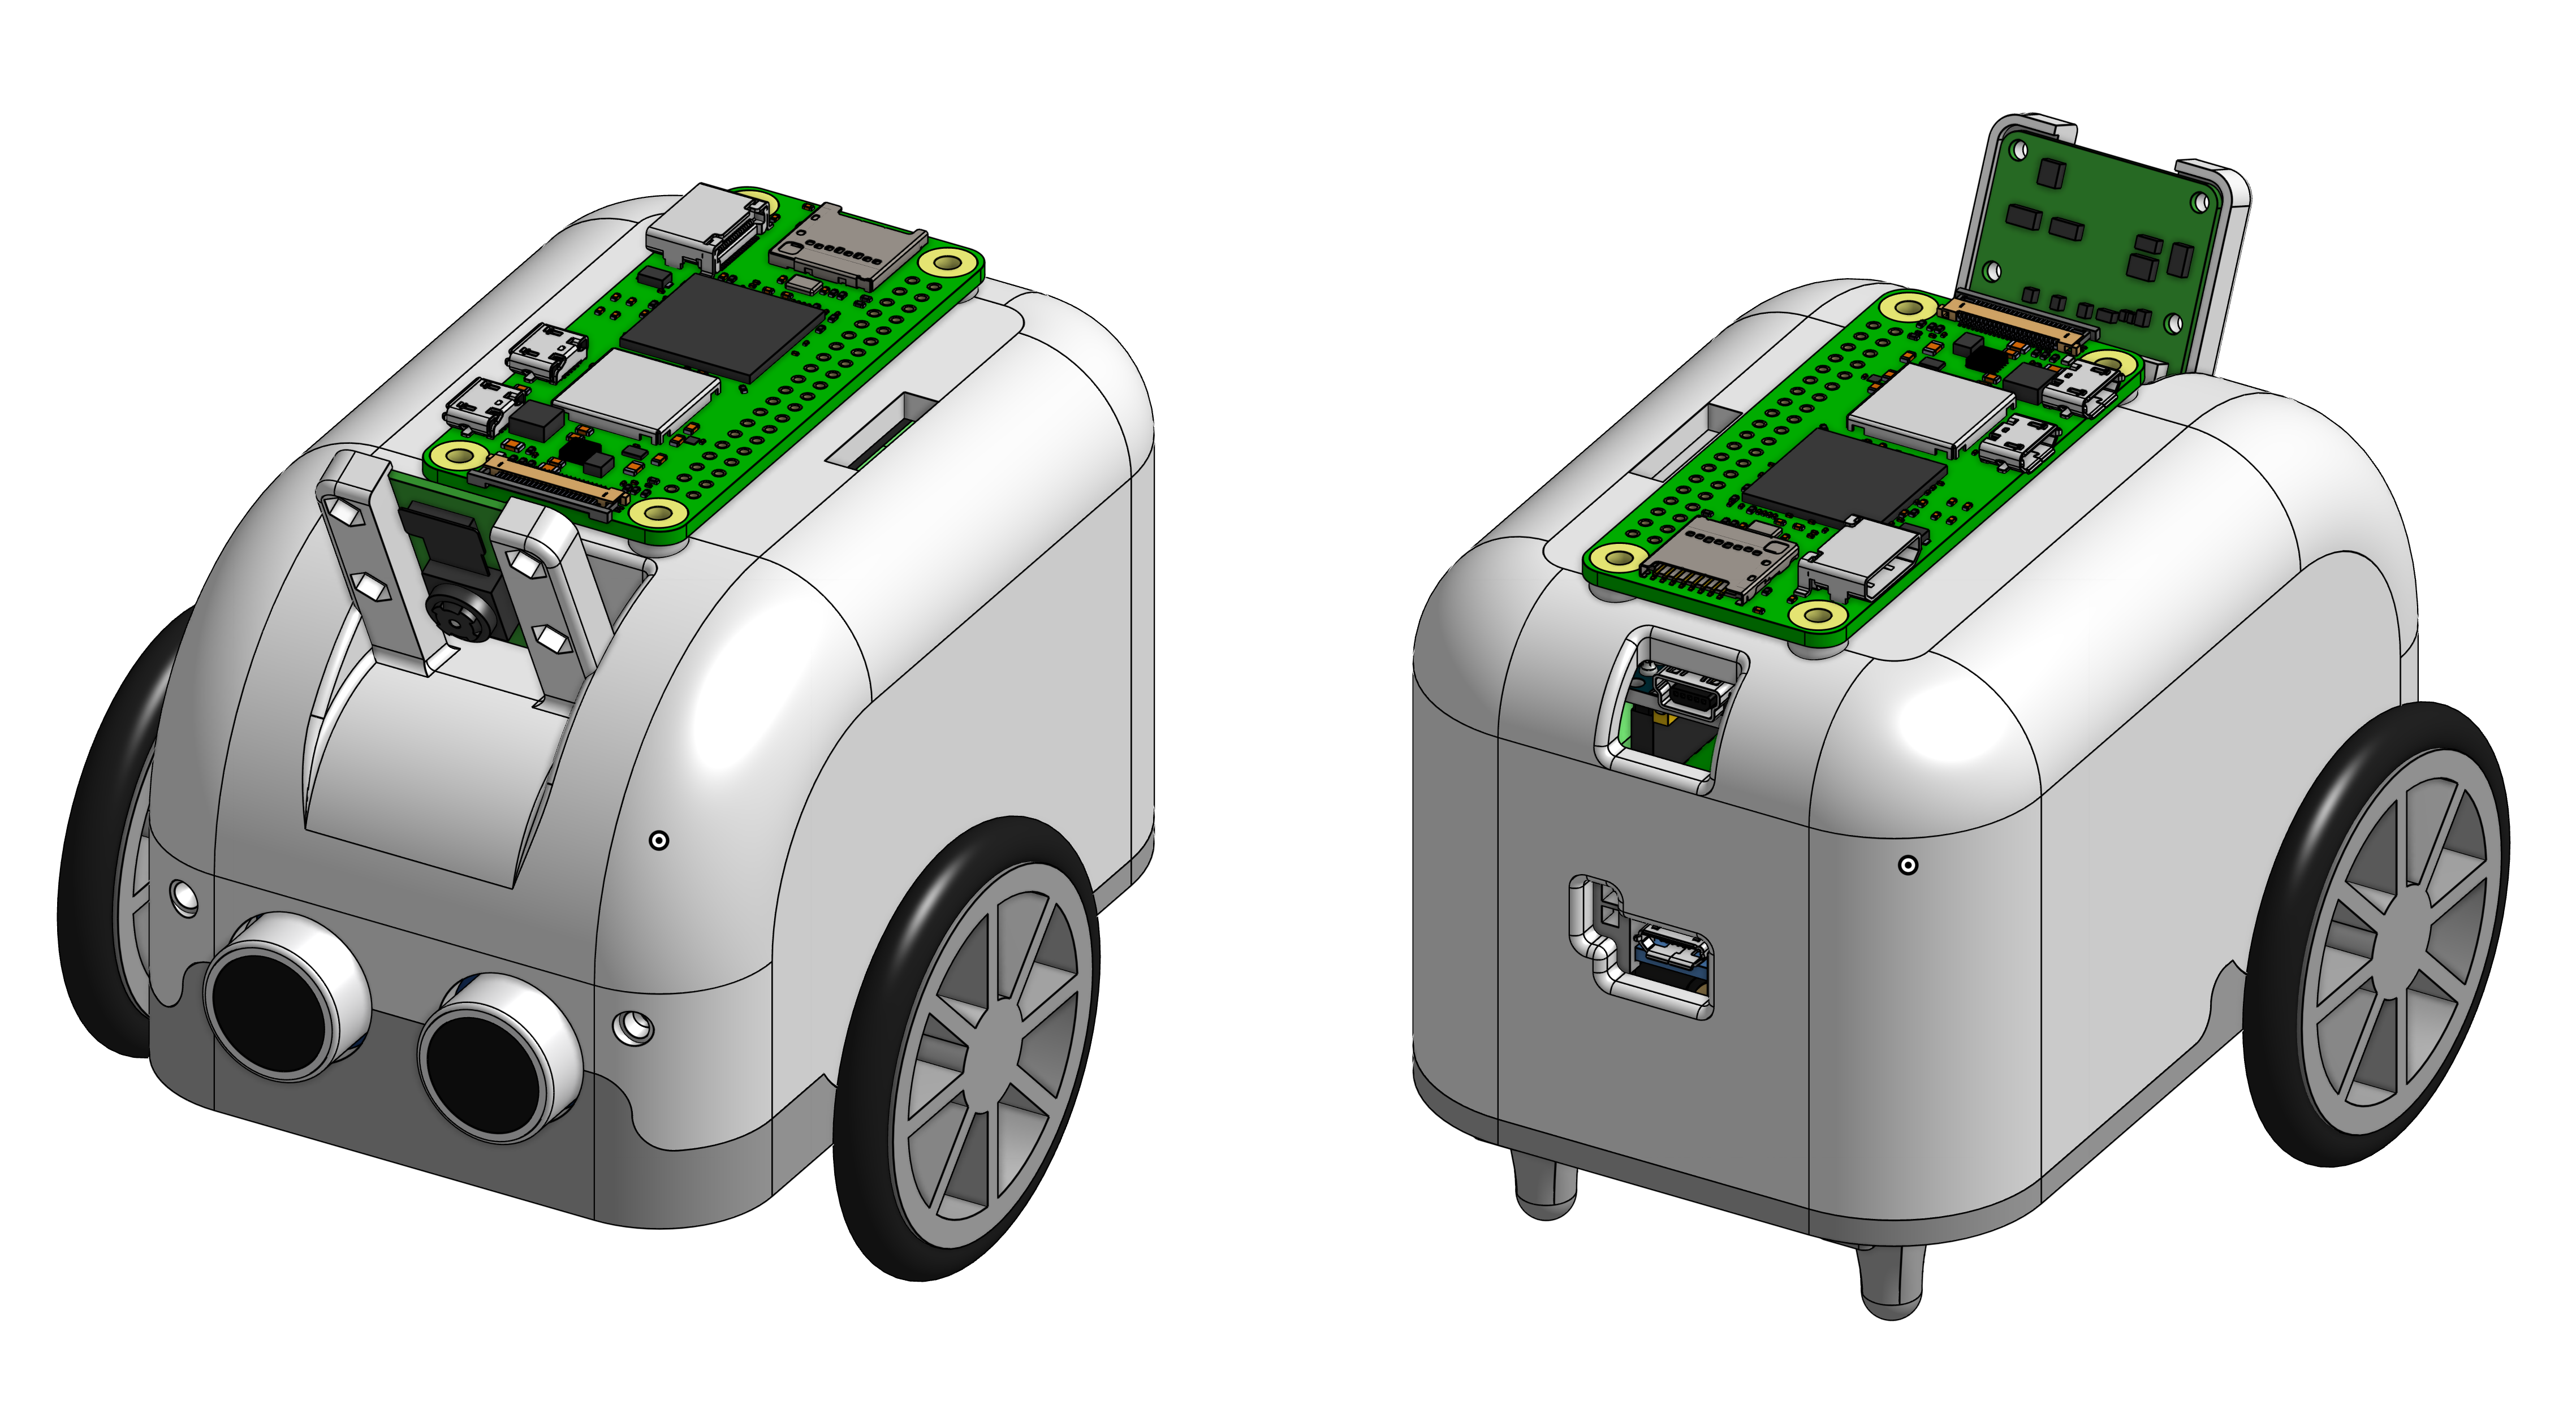
\includegraphics[width=\linewidth]{model_vse}
		\caption{Zakrytované auto s rozšiřujícími moduly (Raspberry Pi)}
		\label{fig:model_vse}
	\end{figure}
	
	% Software
	\newpage
	\section{Software}
	\begin{tabular}{|c|c|c|c|}
		\hline
		g 			\\
		get a value	\\
		\hline
		s 			\\
		set a value \\
		\hline
	\end{tabular}
	
\end{spacing}

\end{document}
% Konec dokumentu